%
% Ostbayerische Technische Hochschule Regensburg (OTH)
% Fakultät Maschinenbau
% Prof. Dr.-Ing. Marcus Wagner
%
% Vorlage und Hinweise für die Erstellung von Abschlussarbeiten
% Inhaltliche Angaben basieren zum Teil auf Vorlagen von Prof. Ehrlich LFT
%
% v7 19.02.2026
\documentclass[
12pt, %Schriftgröße
paper=a4,%Papierformat
%fleqn,%
oneside,% vermeidet Leerseiten, NUR für PDF Ausgabe geeignet, nicht für Ausdruck
%twoside, % WICHTIG: Für Papierausdruck einschalten
DIV=15,BCOR=10mm, % Seitenlayout wie bei Koma-Script
headsepline,%
cleardoublepage=empty, % Keine headsepline auf leeren Seiten, %cleardoublepage=current,%fügt Seitennummer und headsepline ein
headings=normal,%
titlepage,%
bibliography=totoc,% Literaturverzeichnis erscheint im Inhaltsverzeichnis
listof=totoc,% Listen in Inhaltsverzeichnis
parskip=half% s. weiter unten
]{scrbook}  % double sided document
%
%
%-----------------------------------------------------------------------
% HINWEIS zur Übersetzung: Das Dokument kann mit pdflatex/lualatex/xetex übersetzt werden.
%
%Für die Literaturverwaltung muss biber.exe verwendet werden, nicht bibtex.
%-----------------------------------------------------------------------
%
%
%\usepackage{blindtext} % Paket zum Erzeugen von Blindtext zum testen: \blindmathtrue, \blindtext[15], \blinddocument, \Blinddocument, \blindlist{itemize}[5]

%-----------------------------------------------------------------------
% Paketdefinitionen
%-----------------------------------------------------------------------
% --- Engine-Erkennung (pdfLaTeX / LuaLaTeX / XeLaTeX)
\usepackage{iftex}

\ifPDFTeX
% ===== pdfLaTeX =====
\usepackage[utf8]{inputenc} % Eingabe-Encoding (nur für pdfLaTeX nötig)
\usepackage[T1]{fontenc}    % Font-Encoding für korrekte Trennung/Umlaute
\usepackage{lmodern}        % Latin Modern als Schrift
\else
% ===== LuaLaTeX oder XeLaTeX =====
\usepackage{fontspec}       % System/OpenType-Schriften
\defaultfontfeatures{Ligatures=TeX}

% --- Beispiel 1: "Times"-Look (sehr verbreitet) ---
%\setmainfont{TeX Gyre Termes}      % Times-ähnlich, fast immer vorhanden
%\setsansfont{TeX Gyre Heros}       % Helvetica-ähnlich
%\setmonofont{TeX Gyre Cursor}      % Courier-ähnlich

% --- Alternativ: echte Systemfonts (wenn installiert) ---
% \setmainfont{Times New Roman}
% \setsansfont{Arial}
% \setmonofont{Consolas}

% Eine gute Standard-Schrift (ähnlich zu Latin Modern):
%\setmainfont{Latin Modern Roman}
%\setsansfont{Latin Modern Sans}
%\setmonofont{Latin Modern Mono}

\fi

% --- Sprach-/Typo-Pakete (für alle Engines gleich gut)
\usepackage[ngerman]{babel} %Einbindung von neuer Rechtschreibung, deutscher Trennung etc.  babel makes sure the correct hyphenation patterns are used and changes the language of text strings like Table of Contents
\usepackage{csquotes} %Biblatex braucht das. Dient für korrekte Anführungszeichen


\usepackage{microtype} %optimiert den Textsatz auf Mikro‑Ebene, also dort, wo TeX normalerweise sehr starr ist. 

\usepackage{latexsym,amsfonts,amssymb,amsmath,bm} % Standardpakete for mat. Symbole
\usepackage{graphicx} % graphic package of tex
\usepackage{xurl} % Optional: bessere URL-Zeilenumbrüche
\usepackage{array}
\usepackage{longtable} %Tabellen über eine Seite 
\usepackage[per-mode=symbol,exponent-product=\cdot, output-decimal-marker={,}]{siunitx} %Angeben von Einheiten mit Befehl \si{}{}, ang, num, Option per-mode=fraction stellt Brüche sauber dar.
\usepackage[format=hang]{caption}
\usepackage{xcolor} %Farbe orange, Mischen von Farben
\usepackage{subfig}
\usepackage{here} % disables a flow of pictures and can be used with [H]
%\usepackage{mcode} % allows the direct input of m-files




\usepackage{scrhack}
\usepackage{gauss}
\usepackage{tikz}
\usepackage{amssymb}
\usetikzlibrary{decorations.pathmorphing, arrows.meta, patterns}
\usetikzlibrary{shapes,arrows,quotes}
\usepackage{setspace}

\usepackage[
%plainpages=false,
%pdfpagelabels,
raiselinks, pageanchor, hyperindex,
pdftex,
colorlinks=true,
linkcolor=blue,
citecolor=red,
filecolor = black,
urlcolor = blue,
%hidelinks, %Alternativ zu colorlinks, wenn man die Links nicht sehen will 
bookmarks=true,
bookmarksopen=true,
bookmarksopenlevel=2,
pagebackref=false,
bookmarksnumbered=true,
pdfstartpage=1,
pdfstartview=FitH,
plainpages=false,
pdfpagemode=UseOutlines,
]{hyperref}
% for one-sided view in PDF-Reader
\hypersetup{pdfpagelayout=SinglePage,pdfstartview=Fit} 
% for book-like two-sided view in PDF-Reader
%\hypersetup{pdfpagelayout=TwoPageRight} 


%-----------------------------------------------------------------------
% Einbindung Literatur über biblatex
%-----------------------------------------------------------------------
\usepackage[
backend=biber,
style=numeric-comp, %Referenzen sind Zahlen
maxbibnames=99, %Anzahl Namen in Lizverzeichnis bei einem Artikel
date=year,
%maxcitenames=2, %Anzahl genannter Namen bei Zitaten im Text, ohne Angabe maximal drei 
isbn=false, %keine ausgabe, auch wenn in bib enthalten
url=false, %keine ausgabe, auch wenn in bib enthalten
doi=true, %ausgabe,  wenn in bib enthalten. DOI ist sehr wichtig
giveninits=true % Vornamen nur als Initialen
]{biblatex}% !! ACHTUNG muss mit biber übersetzt werden und nicht mit bibtex!
\AtEveryBibitem{\clearfield{pagetotal}} %Ausschalten Ausgabe Feld Seitenzahl
\AtEveryBibitem{\clearlist{language}} %Ausschalten Ausgabe Feld Sprache
\AtEveryBibitem{\clearfield{note}} %Ausschalten Ausgabe Feld Note
\addbibresource{literatur.bib} % Bib Datei mit Einträgen, geht nur in Präambel


%-----------------------------------------------------------------------
% Abkürzungsverzeichnis, Formelzeichen etc. mit glossaries
%-----------------------------------------------------------------------
\usepackage[ 
nonumberlist, %keine Seitenzahlen anzeigen 
acronym,      %ein Abkürzungsverzeichnis erstellen, dafür ist dann keine eigene Definition mit newglossary notwendig
toc=false,          %Einträge im Inhaltsverzeichnis 
nopostdot,    %Kein Punkt am Ende der Beschreibung
nomain,       %Das Hauptglossary wird nicht benutzt
style=super,
section      %im Inhaltsverzeichnis auf section-Ebene erscheinen 
]{glossaries}
%Anlegen von Typen von Glossaren. Vorgegeben sind die Üblochen
%Formelzeichen
\newglossary[slg]{symbolslist}{syi}{syg}{Formelzeichen} 
%Indizesverzeichnis
\newglossary[ilg]{indexlist}{iyi}{iyg}{Indizes} 
%Operatoren und Symbole
\newglossary[olg]{operatorlist}{oyi}{oyg}{Operatoren und Symbole} 
%Glossar erzeugen
\makeglossaries %sorgt dafür, dass die Hilfsdateien angelegt werden.
%
% Das Glossar entsteht an der Stelle wo \printglossaries ausgeführt wird. In diesem Dokument ganz am Ende, siehe unten
%
% WICHTIG, wie Literatur und Index wird Glossar nur durch Ausführen eines eigenen Programms erzeugt
% Dazu In Texstudio Tools->Glossary ausführen (F9-Taste)
% Dafür ist auf dem Rechner eine PERL Installation notwendig.
%
% Die Glossareinträge stehen in dieser Datei. Es muss unbedingt vor begin{document} eingelesen werden
%

%Befehle für Abkürzungen
\newacronym{FEM}{FEM}{Finite-Elemente-Methode}
\newacronym{BEM}{BEM}{Randelementmethode}

%Eintrag in Symbole
\newglossaryentry{symb:u}{
name=$\bm u$,
description={Verschiebungsvektor},
type=symbolslist
}

%Eintrag in Indizes
\newglossaryentry{index:j}{
name=$\textsf{J}$,
description={Knoten $\textsf{J}$ eines Elements},
type=indexlist
}

%Eintrag in Indizes
\newglossaryentry{index:i}{
name=$\textsf{I}$,
description={Knoten $\textsf{I}$ eines Elements},
type=indexlist
}


%Eintrag in Operatorliste
\newglossaryentry{testlist2}{
name=$\nabla$,
description={Gradient},
type=operatorlist
}
\newglossaryentry{testlist}{
name=$\bm{D}_{\varepsilon}()$,
description={Differentialoperatormatrix},
type=operatorlist
}

\glsaddall %Auch ohne Nutzung im Text werden alle Inhalte ausgegeben





%
%Nutzung des Glossar, z.B \gls{FEM}. Dies führt bei der ersten Nutzung dazu, dass die Abkürzung ausgeschrieben wird, bei weiterer Nutzung nur noch die Abkürzung.


%-----------------------------------------------------------------------
% Layout
%-----------------------------------------------------------------------
%\textwidth		 160mm % in Word 2,5cm Rand jede Seite, also 16cm Breite
%\textheight 	 252mm % in Word 2,5 oben, 2 unten, also Höhe 252
%\oddsidemargin   6mm
%\evensidemargin -6mm
%\topmargin      -12mm
%%\headheight     0cm
%\headsep    	 5mm
%\topskip    	 0mm
%\voffset    	 0mm
%\hoffset    	 0mm
%\footskip   	 7.5mm
%\raggedbottom
%\renewcommand{\topfraction}{1.0}
%% Explizites Setzen Zeilenabstand bei Absatz, parskip=half sehr groß
\setlength{\parskip}{2ex plus 0.5ex minus 0.5ex}

\usepackage{enumitem} %Abstände in Listen einstellen
%\setlist[itemize]{noitemsep, nolistsep} %sehr kompakt
%\setlist[enumerate]{noitemsep, nolistsep}
\setlist{itemsep=1pt, parsep=1pt} % Setzt itemsep auf kleinen Abstand für alle Listen



\usepackage{siunitx}
%-----------------------------------------------------------------------
% Grafikpfad
%-----------------------------------------------------------------------
% Commands for figures:
%\DeclareGraphicsExtensions{.eps,.ai} % file extension of postscript-pictures for the generation of PS-documents
%\DeclareGraphicsExtensions{.pdf,.jpg} % file extension of postscript-pictures for the generation of PDF-documents
\graphicspath{{figs/}} % path of the picture files
\def\figurename{Abb. } % keyword for the captions

%-----------------------------------------------------------------------
% Kommandos für einheitliche Bezeichnungen im Dokument
%-----------------------------------------------------------------------
\newcommand{\Eqref}[1]{Gl.\,(\ref{#1})}
\newcommand{\Figref}[1]{Abb.\,\ref{#1}}
\newcommand{\Chapref}[1]{Kap.\,\ref{#1}}
\newcommand{\Anhref}[1]{Anh.\,\ref{#1}}
\newcommand{\Tabref}[1]{Tab.\,\ref{#1}}

\newcommand{\RNum}[1]{\uppercase\expandafter{\romannumeral #1\relax}}

%-----------------------------------------------------------------------
%-----------------------------------------------------------------------
% Beginn Input: Allgemeine Angaben zu Titel und Autor
%-----------------------------------------------------------------------
%-----------------------------------------------------------------------
%
% type of thesis:
%\newcommand{\graduation}{Master} \newcommand{\abbretyp}{M}
\newcommand{\graduation}{Bachelor} \newcommand{\abbretyp}{B}
%
% Choose ONE of the following programms:
%\newcommand{\studies}{Produktions- und Automatisierungstechnik}
\newcommand{\studies}{Maschinenbau} \newcommand{\abbrestud}{MB}
%\newcommand{\studies}{Industrial Engineering} \newcommand{\abbrestud}{IE}
%
% Enter the name of the thesis:
\newcommand{\doctitle}{Einführung eines Standards zur Aufbereitung und Auswertung von Messdaten der Hydropulsanlage}
%---------------------------------- -------------------------------------
% Bei externer Arbeit die folgenden drei Kommandos aktivieren
%---------------------------------- -------------------------------------
% Enter the name of the cooperating company:
\newcommand{\company}{}
% Enter the address of the cooperating company:
%\newcommand{\compaddress}{Traunreutherstra?e 1, 93055 Neutraubling}
% Enter the name of the company advisor:
\newcommand{\betreuer}{}
% Enter the name of the academic advisor:
\newcommand{\professor}{Prof. Dr.-Ing. Marcus Wagner}
% Enter the start date of your work:
\newcommand{\beginndatum}{<16.03.2026>}
% Enter the end date of your work:
\newcommand{\abgabedatum}{16.08.2026}
% Enter how you want to be adressed:
\newcommand{\bearbeiteranrede}{Frau}
% Enter your name:
\newcommand{\bearbeitername}{Carla Hüttner}
\newcommand{\bearbeitergeburtstag}{<01.08.2003>}
% Enter your matriculation number
\newcommand{\matrikelnummer}{<3333699>}

\newcommand{\bearbeitungszeitraum}

% Additional settings for PDF-document:
\hypersetup{
pdftitle=\doctitle,
pdfauthor=\bearbeitername,
pdfsubject=\studies,
% Enter 5-7 keyword for your work/area of work:
pdfkeywords={}
}

% -----------------------------------
% --- Main Document -----------------
% ---               -----------------
%\includeonly{}

\begin{document}

    \pagenumbering{arabic}

    %% Einleitungsseiten, müssen so genutzt werden
    

%-----------------------------------------------------------------------
%-----------------------------------------------------------------------
% Title Page 
%---------------------------------- -------------------------------------
%-----------------------------------------------------------------------
\thispagestyle{empty}
\hypertarget{titelseite}{}
\pdfbookmark[0]{Titelseite}{titelseite}

%Linksbündiger Stil nach OTH WORD Vorlage
%---------------------------------- -------------------------------------
% Logo auswählen
%---------------------------------- -------------------------------------
\vspace*{-2cm}

\includegraphics[width=0.5\textwidth]{othr-logo_flat} \hfill
%\includegraphics*[angle=0, scale=0.4]{OTH_Logo_LMS} \hfill

%\vskip5cm

{\sffamily
\vspace*{2.7cm}
%\begin{center}
    {\Huge \textbf{\MakeUppercase{{\graduation}arbeit}}}
    \vskip1mm

    {\Large \textbf{\bearbeitername}}
    \vskip3.3cm

    \LARGE \textbf{\doctitle} 

    \normalsize

    \vfill

    \begin{tabular}{ll}
        Fakultät: & Maschinenbau\\
        Studiengang: & \studies~(\abbretyp-\abbrestud)\\
        Abgabedatum:& \abgabedatum\\
        Aufgabensteller: & \professor{}\\
        %---------------------------------- -------------------------------------
        % Bei externer Arbeit aktivieren
        %---------------------------------- -------------------------------------
   
        %		Beginn:& \beginndatum \\
    \end{tabular}
%\end{center}

%\vfill 

}

%Leerseite einfügen
\cleardoublepage

%---------------------------------- -------------------------------------
%---------------------------------- -------------------------------------
% Geheimhaltung falls notwendig
%---------------------------------- -------------------------------------
%---------------------------------- -------------------------------------
\thispagestyle{empty}

%\scalebox{1.25}
%\hspace*{-2cm}{\includegraphics[width=1.0\textwidth]{Geheimhaltungsverpflichtung bei Betreuung einer Abschlussarbeit.pdf}}\label{p:ghv}
%Leerseite einfügen
\cleardoublepage


%---------------------------------- -------------------------------------
%---------------------------------- -------------------------------------
% Erklärung
%---------------------------------- -------------------------------------
%---------------------------------- -------------------------------------


\includepdf[pages=-]{Erklaerung.pdf}


%Leerseite einfügen
\cleardoublepage

%---------------------------------- -------------------------------------
%---------------------------------- -------------------------------------
% Abstract 
%---------------------------------- -------------------------------------
%---------------------------------- -------------------------------------
%\thispagestyle{empty}
{\LARGE\textsf{\textbf{Kurzfassung}}}
\vskip0.5cm

\relax
Im Rahmen dieser Bachelorarbeit wurde eine MATLAB-basierte Auswertesoftware zur standardisierten Aufbereitung und Auswertung von Messdaten aus Schwingfestigkeitsversuchen an einer Hydropulsanlage entwickelt. Ziel war es, die bisher erforderlichen manuellen Auswertungsschritte zu vereinheitlichen und weitgehend zu automatisieren.

Die entwickelte Software ermöglicht das Einlesen und die automatisierte Aufbereitung der für die Auswertung relevanten Messdaten. Anschließend werden der Zeit- und Langzeitfestigkeitsbereich auf Grundlage der DIN 50100 statistisch ausgewertet und die zugehörigen Wöhlerlinien für unterschiedliche Ausfallwahrscheinlichkeiten bestimmt.

Die Anwendung der Auswertesoftware wird anhand realer sowie zusätzlich erstellter fiktiver Versuchsdaten demonstriert. Aus den aufgezeichneten Messdaten konnten die erforderlichen Kennwerte bestimmt und daraus die Wöhlerlinien für Ausfallwahrscheinlichkeiten von 10\,\%, 50\,\% und 90\,\% erstellt werden. Die Auswertung lieferte plausible Ergebnisse und bestätigte damit die Funktionsfähigkeit der entwickelten Software. Abschließend werden die Versuchsergebnisse automatisiert in einem PDF-Prüfprotokoll auf Basis einer LaTeX-Vorlage dokumentiert. Insgesamt ermöglicht die entwickelte Auswertesoftware einen einheitlichen und nachvollziehbaren Ablauf von der Messdatenaufbereitung über die statistische Auswertung bis hin zur Darstellung und Dokumentation der Versuchsergebnisse.
\vfill
{\LARGE\textsf{\textbf{Abstract}}}
\vskip0.5cm
\relax
As part of this bachelor's thesis, a MATLAB-based evaluation software was developed for the standardised preparation and analysis of measurement data from fatigue tests on a hydraulic pulse testing machine. The objective was to standardise and largely automate the manual evaluation steps previously required. 

The developed software enables the importing and automated preparation of the measurement data relevant to the evaluation. Subsequently, the high-cycle and long-life fatigue regimes are statistically evaluated on the basis of DIN 50100, and the corresponding S-N curves are determined for different failure probabilities. 

The application of the evaluation software is demonstrated using real as well as additionally generated fictitious test data. The required characteristic values were determined from the recorded measurement data, and the S-N curves for failure probabilities of 10\,\%, 50\,\% and 90\,\% were generated from them. The evaluation yielded plausible results, thereby confirming the functionality of the developed software. Finally, the test results are automatically documented in a PDF test report based on a LaTeX template. Overall, the developed evaluation software enables a uniform and traceable process from measurement data preparation and statistical evaluation to the presentation and documentation of the test results.


\vfill
%Leerseite einfügen
\cleardoublepage

% -----------------------------------
% ---  table of contents is created
% ---          ----------------------
\setcounter{tocdepth}{2}
\tableofcontents % a table of contents is created

%\vfill
%Leerseite einfügen
\cleardoublepage


%Glossar ausgeben
%\printglossary[title=Glossar] %Allgemeines, vordefiniertes GLossar, hier nicht genutzt 
%\printglossary[type=\acronymtype,style=long,title=Abkürzungsverzeichnis] 
%\printglossary[type=symbolslist,style=long] 
%\printglossary[type=indexlist,style=long] 
%\printglossary[type=operatorlist] 

\vfill
%Leerseite einfügen
\cleardoubleemptypage




    %Auf Wunsch, für die Bewertung hat dies keine Auswirkungen
    %\listoffigures % a list of all figures is created
    %\listoftables % a list of all tables is created

    %% Kapitel

    %
%-----------------------------------------------------------------------
\chapter{Einleitung}%\label{chap:kap1}
%-----------------------------------------------------------------------
    %-----------------------------------------------------------------------
    \section{Stand der Technik} %\label{chap:sec1}
 Durch die Industrialisierung des 19. Jahrhunderts, insbesondere durch die Entwicklung der Eisenbahn und deren Schadensfälle hat August Wöhler mit Versuchen eine neue Technik zur Lösung von zahlreichen Problemen entwickelt. Er hat durch gebrochene Radsatzwellen an Lokomotiven entdeckt, dass Bauteile auch unterhalb der statischen Festigkeitsgrenze beschädigt werden können. 
Sein Versuch, der den Zusammenhang zwischen Bruchlastspielzahl und Ausschlagspannung herstellt zeigt, dass wiederholte, schwingende Belastungen zum Bruch führen können, auch wenn sie weit unterhalb der statischen Festigkeitsgrenze liegen.
Seitdem spielt die dynamische Werkstoffprüfung eine wichtige Rolle und befindet sich mittlerweile im alltäglichen Gebrauch von Firmen.


    %	
    %-----------------------------------------------------------------------
    \section{Motivation} %\label{chap:sec1}
    %-----------------------------------------------------------------------
Die vorliegende Bachelorarbeit dient der Entwicklung einer MATLAB-Auswertesoftware, die die Belastung der Maschine und die Reaktion des Prüflings bewertet. Der komplette Aufgabenbereich ist interessant und spannend, weil er von der Funktion und Bedienung der Anlage bis zum Kundenauftrag mit zertifizierten Prüfschein reicht.  






    \chapter{Theoretischer Hintergrund}

	\section{Werkstoffmechanische Grundlagen der Ermüdung}
	
Wird ein statischer Lastfall betrachtet, bilden die Zugfestigkeit, definiert als die Maximalspannung, die ein Werkstoff ertragen kann, sowie die Streckgrenze die zentralen Kenngrößen  \cite[Seite 117]{HibbelerTechnischeMechanik2013}. 

Wenn die wirkende Spannung geringer als die Streckgrenze ist, verformt sich das Bauteil elastisch. Überschreitet die Spannung diese Grenze, tritt neben der elastischen auch eine makroskopische plastische Verformung auf \cite[Seite 8]{Laepple2016}. Unter zyklischer Belastung hingegen treten plastische Verformungen in der Mikrostruktur des Metalls bereits weit unterhalb der Streckgrenze auf. Das Voranschreiten dieser mikrostrukturellen Schädigung wird als Materialermüdung bezeichnet. Dieser Prozess kann schlussendlich zu einem Ermüdungsbruch führen \cite[Seite 1-5]{Ermüdungsfestigkeit2007}.  

Die mechanische Spannung ist das Verhältnis aus der inneren Kraft bezogen auf die beanspruchte Querschnittsfläche \cite[Seite 9-10]{Balke2008}. Der Spannungsbegriff wird in die Normalspannung und die Tangentialspannung unterteilt, die sich durch die Richtung der Krafteinwirkung bezüglich der betrachteten Fläche voneinander unterscheiden. Normalspannungen entstehen durch senkrecht auf die Fläche auftretende Kräfte. Tangentialspannungen hingegen ergeben sich immer dann, wenn Kräfte in der Schnittebene wirken, die beispielsweise durch äußere Querkräfte $F_Q$ hervorgerufen werden~\cite[Seite 206]{KabusFestigkeitslehre2023}. 
Im elastischen Fall bewegt sich das Bauteil nach Entlastung wieder in die Ausgangslage zurück. Unter zyklischer Belastung hingegen führen wiederholte, mikroplastische Verformungen zu einer irreversiblen Schädigung, welche die die Grundlage für die spätere Materialermüdung und Rissentstehung bildet \cite[Seite 8]{Laepple2016} \cite[Seite 5]{Ermüdungsfestigkeit2007}. 

	\subsection{Mikroskopische Rissentstehung (Gitterfehler)}
Metalle liegen als Realkristalle vor, die sich durch ihre fehlerhafte Gitterstruktur auszeichnen. Diese Defekte lassen sich anhand ihrer räumlichen Dimension in nulldimensionale (punktförmige), eindimensionale (linienförmige), zweidimensionale (flächenhafte) und dreidimensionale (räumliche) Gitterfehler klassifizieren. Zu den nulldimensionalen Defekten gehören Leerstellen, Substitutions- und Zwischengitteratome. Die Gruppe eindimensionaler Defekte umfasst die Stufen- und Schraubenversetzungen. Zweidimensionale Defekte sind zum Beispiel Korngrenzen und Stapelfehler. \\
Zu den dreidimensionalen Defekten gehören Poren, Einschlüsse und Ausscheidungen \cite[Kapitel 2.2.1]{Werkstoffkunde2015}. Die Entstehung von Ermüdungsrissen basiert auf dem Vorhandensein von Leerstellen und der Bewegung von Versetzungen.

Bei idealen Kristallen ist jeder Platz in der Gitterstruktur mit einem Atom belegt. Ein Realkristall hingegen weist unbesetzte Gitterplätze auf. Diese ermöglichen die Diffusion der Atome und je mehr Leerstellen vorhanden sind, umso höher ist das Ausmaß der Diffusion. Hierdurch wird die plastische Verformung begünstigt, da durch die Leerstellen das Klettern von Versetzungen erfolgen kann. Durch die plastische Verformung eines Bauteils verstärkt sich dieser Effekt zunehmend. \cite[Kapitel 2.2.1]{Werkstofftechnik2018}.

Die Versetzungsbewegung tritt ein, wenn die auf das Gleitsystem einwirkende Schubspannung größer ist als die kritische Schubspannung des Werkstoffs. Die Versetzungen wandern bis zu einem Hindernis, wie etwa einer Korngrenze oder Ausscheidungen. \\ 
Als Grundlage für die plastische Verformung bei zyklischer Beanspruchung dient eine geringe Anzahl an Versetzungen, die sich unter der Streckgrenze bereits bewegen können. Wenn sich die Versetzungen an Korngrenzen aufstauen, erzeugt dies Spannungen im Nachbarkristall und es können sich infolgedessen auch dort Versetzungen bewegen. In der Belastungsphase entsteht durch das Wandern der Versetzungen eine Gleitverschiebung~($\Delta s$). Dabei entsteht eine neue Oberfläche. Durch Oxidation an der neuen Oberfläche wird die Gleitebene blockiert. Um bei Lastumkehr wieder in die andere Richtung wandern zu können, erfolgt die Rückgleitung der Versetzungen auf einer parallelen Gleitebene, dargestellt in Teilbild b) in \Figref{fig:gleitbaender-mechanismus}. Mit jedem Belastungszyklus wiederholt sich dieser Vorgang und es entstehen an der Oberfläche Intrusionen und Extrusionen \cite[Seite 265-267]{Werkstofftechnik-Praktikum2021}. 

\begin{figure}[H] 
    \centering
\begin{tikzpicture}[scale=0.8, every node/.style={scale=0.8}]
    \tikzset{
        oberflaeche/.style={ultra thick},
        gleitlinie/.style={thin},
        gleitband_rand/.style={thick},
        spannungskurve/.style={thick}
    }

    \foreach \x / \label / \stage in {0/a/1, 3.5/b/2, 7/c/3, 10.5/d/4, 14/e/5} {
        \begin{scope}[xshift=\x cm]
            % Gestrichelter Rahmen rechts
            \draw[dashed] (1,0) -- (2.5,0) -- (2.5,5) -- (1,5);
            
            % --- Geometrie ---
            \ifnum \stage=1 % a)
                \draw[oberflaeche] (0.5,0) -- (0.5,2); 
                \draw[thick] (0.5,2) -- (0.8,2.3); 
                \draw[oberflaeche] (0.8,2.3) -- (0.8,5); 
                \draw[gleitband_rand] (0.5,2) -- (2.5,4);
                \draw[->] (1.2, 3.0) -- (1.6, 3.4) node[midway, sloped, above=0.1cm] {$\Delta s$};
                \draw[<-] (0.8, 4) -- (-0.2, 4) node[left, align=right] {Oberfläche\\alt};
                \draw[<-] (0.65, 2.15) -- (-0.2, 2.15) node[left, align=right] {neu};
                \draw[->, thick] (1.5, 5.2) -- (1.5, 5.8) node[right] {$\sigma$};
            \fi

            \ifnum \stage=2 % b)
                \draw[oberflaeche] (0.5,0) -- (0.5,1.6);
                \draw[oberflaeche] (0.5,1.9) -- (0.5,5);
                \draw[thick] (0.5,1.6) -- (0.7,1.8); 
                \draw[thick] (0.7,1.77) -- (0.7,2.1); 
                \draw[thick] (0.7,2.1) -- (0.5,1.9); 
                \draw[gleitband_rand] (0.7,1.79) -- (2.5,3.59); 
                \draw[gleitband_rand] (0.7,2.1) -- (2.5,3.9); 
                \draw[->, >=stealth] (1.5, 3.3) -- (1.1, 2.9); 
            \fi

            \ifnum \stage=3 % c) KORREKTUR: Wand zurück auf x=0.7, kleiner Strich nach rechts verschoben
                \draw[oberflaeche] (0.5,0) -- (0.5,1.6); % Untere Wand
                \draw[oberflaeche] (0.7,2.0) -- (0.7,5); % Obere Wand bleibt bei 0.7
                
                % Schräge Verbindungslinie (Top)
                \draw[thick] (0.7,2.0) -- (2.5,3.8); 
                
                % Kleine Linie verschoben: Schräge zu x=0.85, vertikaler Strich bei 0.85
                \draw[thick] (0.5,1.6) -- (0.85,1.9); 
                \draw[thick] (0.85,1.9) -- (0.85,2.02); % Der verschobene kleine Strich
                \draw[thick] (0.9,2.05) -- (0.9,2.2);  % Schräge zurück zur Wand
                
                % Gleitbänder (starten am verschobenen Strich)
                \draw[gleitband_rand] (0.85,1.9) -- (2.5,3.55); %unterste linie
                \draw[gleitband_rand] (0.85,2.02) -- (2.5,3.67);
                \draw[->] (1.3, 3.0) -- (1.7, 3.4);
            \fi

            \ifnum \stage=4 % d)
                \draw[oberflaeche] (0.5,0) -- (0.5,1.6);
                \draw[oberflaeche] (0.5,1.9) -- (0.5,5);
                \draw[thick] (0.5,1.6) -- (0.7,1.8) -- (0.7,1.9) -- (0.8,2.0) -- (0.8,2.1) -- (0.9,2.2) -- (0.9,2.3) -- (0.5,1.9);
                \draw[gleitband_rand] (0.7,1.8) -- (2.5,3.6);
                \draw[gleitband_rand] (0.7,1.9) -- (2.5,3.7);
                \draw[gleitband_rand] (0.8,2.0) -- (2.5,3.7);
                \draw[gleitband_rand] (0.8,2.1) -- (2.5,3.8);
                \draw[gleitband_rand] (0.9,2.2) -- (2.5,3.8);
                \draw[gleitband_rand] (0.9,2.3) -- (2.5,3.9);
                \node[rotate=45, anchor=south] at (1.7,2.0) {Gleitband};
                \node[anchor=south west] at (0.6,0.3) {Intrusion};
                \draw[<-] (1.2, 3.0) -- (1.6, 3.4);
            \fi

            \ifnum \stage=5 % e)
                \draw[oberflaeche] (0.5,0) -- (0.5,1.6);
                \draw[oberflaeche] (0.5,1.9) -- (0.5,5);
                \draw[thick] (0.5,1.6) -- (0.2,1.3) -- (0.2,1.6) -- (0.5,1.9);
                \draw[gleitband_rand] (0.2,1.3) -- (2.5,3.6);
                \draw[gleitband_rand] (0.2,1.6) -- (2.5,3.9);
                \node[anchor=south west] at (0.45,0.3) {Extrusion};
            \fi

            % --- Diagramme ---
            \ifnum \stage<5
            \begin{scope}[yshift=-1.8cm, scale=0.6, xshift=0.5cm]
                \draw[->] (0,0) -- (2.5,0) node[right] {$t$};
                \draw[->] (0,0) -- (0,1.5) node[above] {$\sigma$};
                \ifnum \stage=1 \draw[spannungskurve] (0.5,0) .. controls (1,0) and (1,1) .. (1.5,1); \fi
                \ifnum \stage=2 \draw[spannungskurve] (0.1,0) .. controls (0.4,0) and (0.4,1.2) .. (0.7,1.2) .. controls (1.0,1.2) and (1.0,0) .. (1.3,0); \fi
                \ifnum \stage=3 \draw[spannungskurve] (0.1,0) .. controls (0.4,0) and (0.4,1.2) .. (0.7,1.2) .. controls (1,1.2) and (1,0) .. (1.3,0) .. controls (1.6,0) and (1.6,1.2) .. (1.9,1.2); \fi
                \ifnum \stage=4 \draw[spannungskurve] (0.1,0) .. controls (0.4,0) and (0.4,1.2) .. (0.7,1.2) .. controls (1,1.2) and (1,0) .. (1.3,0) .. controls (1.6,0) and (1.6,1.2) .. (1.9,1.2) .. controls (2.2,1.2) and (2.2,0) .. (2.5,0); \fi
            \end{scope}
            \fi
            
            \node at (1.25,-2.7) {(\label)};
        \end{scope}
    }

\end{tikzpicture}
    \caption{Entstehung von Gleitbändern, sowie Intrusionen und Extrusionen infolge zyklischer Beanspruchung (In Anlehnung an \cite[Seite 8]{Ermüdungsfestigkeit2007}).}
    \label{fig:gleitbaender-mechanismus}
\end{figure}

Zusammengefasst ist die Grundlage der plastischen Verformung die Versetzungsbewegung, die dann zu Intrusionen und Extrusionen führt, an denen sich Risskeime ausbilden und ein Anriss entsteht. 

Der Rissvorgang bildet sich oftmals zuerst an den Intrusionen aus. Bei der zyklischen Beanspruchung wird der Riss bei jedem Lastwechsel geöffnet und dann wieder weitestgehend geschlossen, wodurch dieser bei jedem Zyklus wächst. 

Insgesamt werden drei Rissstadien unterschieden: Im Rissstadium 1 (siehe \Figref{fig:Rissausbreitung}) entstehen solange Anrisse, bis die Spannungsspitzen im Kerbgrund derart fortgeschritten sind, sodass sich das Bauteil nicht mehr weiter plastisch verformen kann und der Riss umschwenkt. Die Ausbreitung geschieht dabei senkrecht zur größten Normalspannung (=~Rissstadium 2). \Figref{fig:Rissausbreitung} veranschaulicht diese Richtungsänderung. Die Rissausbreitung verläuft transkristallin durch die einzelnen Körner hindurch. 

\begin{figure}[H]
\centering
\begin{tikzpicture}[scale=1.3, every node/.style={scale=0.9}]

    % --- 1. Gefügehintergrund (Graue Fläche mit Zackenrand oben/unten) ---
    \fill[gray!60] (0,0.5) -- (0.5,0.7) -- (1,0.5) -- (1.5,0.6) -- (2,0.4) -- (2.5,0.6) -- (3,0.5) -- (3.5,0.7) -- (4,0.5) -- (4.5,0.6) 
                -- (4.5,4.4) -- (4,4.5) -- (3.5,4.3) -- (3,4.5) -- (2.5,4.4) -- (2,4.6) -- (1.5,4.4) -- (1,4.5) -- (0.5,4.3) -- (0,4.5) -- cycle;

    % --- 2. Korngrenzen (Weiße Linien im Gefüge) ---
    \tikzset{korngrenze/.style={white, thick}}
    \draw[korngrenze] (0,3.8) -- (0.8,3.9) -- (1.4,4.4);
    \draw[korngrenze] (0.8,3.9) -- (1.1,3.2) -- (0,3.0);
    \draw[korngrenze] (1.1,3.2) -- (1.8,3.6) -- (2.5,4.4);
    \draw[korngrenze] (1.8,3.6) -- (2.2,2.9) -- (1.3,2.5) -- (1.1,3.2);
    \draw[korngrenze] (1.3,2.5) -- (0.6,2.3) -- (0,2.1);
    \draw[korngrenze] (0.6,2.3) -- (0.9,1.4) -- (0,1.2);
    \draw[korngrenze] (0.9,1.4) -- (1.7,1.7) -- (2.2,2.9);
    \draw[korngrenze] (1.7,1.7) -- (2.0,0.9) -- (1.1,0.6);
    \draw[korngrenze] (2.0,0.9) -- (3.0,1.2) -- (3.2,2.2) -- (2.2,2.9);
    \draw[korngrenze] (3.2,2.2) -- (4.0,2.6) -- (4.5,2.4);
    \draw[korngrenze] (4.0,2.6) -- (3.8,3.6) -- (4.5,3.9);
    \draw[korngrenze] (3.8,3.6) -- (2.8,3.8) -- (2.5,4.4);
    \draw[korngrenze] (2.8,3.8) -- (3.2,2.2);
    \draw[korngrenze] (3.0,1.2) -- (3.9,0.8) -- (4.5,1.1);
    \draw[korngrenze] (3.9,0.8) -- (4.2,1.9) -- (4.0,2.6);

    % --- 3. Bauteiloberfläche (Dicke schwarze Linie links) ---
    \draw[line width=2.5pt, black] (0,0.5) -- (0,4.5);

    % --- 4. Belastungspfeile (Grau gefüllte Doppelpfeile ohne schwarze Innenlinie) ---
    \tikzset{belastungspfeil/.style={<->, >=latex, line width=3.4pt, gray!80}}
    \draw[belastungspfeil] (2.25,4.6) -- (2.25,5.6);
    \draw[belastungspfeil] (2.25,0.4) -- (2.25,-0.6);

    % --- 5. Risse (Anrisse und Hauptriss) ---
    % Kleine Nebenanrisse links
    \draw[line width=1.8pt, black] (0,4.1) -- (0.5,3.7);
    \draw[line width=1.8pt, black] (0,3.3) -- (0.4,3.1);
    \draw[line width=1.8pt, black] (0,0.9) -- (0.6,1.2);
    
    % Hauptermüdungsriss (Stadium 1 zu Stadium 2)
    % Schräger Verlauf (Stadium 1)
    \draw[line width=2.2pt, black] (0,1.7) -- (2.6,3.4); 
    % Horizontaler Verlauf mit Pfeilspitze (Stadium 2)
    \draw[line width=2.2pt, black, ->, >=stealth] (2.6,3.4) -- (4.2,3.4);

    % --- 6. Stadien-Nummerierung (1 und 2) ---
    \node[font=\small\sffamily] at (0.2,4.2) {1};
    \node[font=\small\sffamily] at (0.5,3.4) {1};
    \node[font=\small\sffamily] at (1.1,2.2) {1};
    \node[font=\small\sffamily] at (4.0,3.1) {2};

    % --- 7. Textbeschriftungen und Hinweislinien ---
    \node[anchor=east, font=\itshape] (txt-oberflaeche) at (-0.3,0.3) {Oberfläche};
    \draw[->, >=latex, thin] (txt-oberflaeche) -- (0,0.5);

    \node[anchor=east, font=\itshape] (txt-anriss) at (-0.3,1.9) {Anriss};
    \draw[->, >=latex, thin] (txt-anriss) -- (0.75,2.25);
    \draw[->, >=latex, thin] (txt-anriss) -- (0.15,3.2);

    \node[anchor=west, font=\itshape] (txt-korngrenze) at (4.3,1.5) {Korngrenze};
    \draw[->, >=latex, thin] (txt-korngrenze) -- (3.1,1.7);

    % Text entlang des Risses rotiert (Zusammengeschrieben: Rissausbreitung)
    \node[rotate=33, font=\small\bfseries\itshape, anchor=south] at (1.4,2.7) {Rissausbreitung};

\end{tikzpicture}
\caption{Rissstadium 1 und 2 (In Anlehnung an \cite[Seite 268]{Werkstofftechnik-Praktikum2021}).}
\label{fig:Rissausbreitung}
\end{figure}

Da die Rissgröße pro Schwingung zunimmt, verringert sich folglich die lasttragende Fläche und die Spannung im Bauteil erhöht sich. Wenn die Spannung im verbleibenden, lasttragenden Querschnitt die Zugfestigkeit erreicht, tritt Rissstadium 3 ein und es erfolgt der Restgewaltbruch \cite[Seite 267-269]{Werkstofftechnik-Praktikum2021}. 

Im Wöhlerversuch führen diese Mikrorisse schließlich zum Versagen des Bauteils. Deshalb wird untersucht, wie viele Lastspiele das Material erträgt, bevor die Summe der Mikrorisse zu einem makroskopischen Riss im Bauteil führt. 
\clearpage


	\section{Scherzugversuch}
Das Ziel des Scherzugversuches ist es, die Maximalkraft $F_{\text{max}}$ zu bestimmen, die die Probe vor ihrem Versagen erträgt \cite[Seite 216-218]{RoloffMatek2021}. Diese Maximalkraft, auch Scherkraft genannt, ist anschließend die oberste Grenze für die Lasthorizonte des nachfolgenden Wöhlerversuches.  

Die zwei Versagensarten, die auftreten können, sind die Abscherung des Niets, durch Überschreiten der Scherspannung im Niet, oder ein Blechriss infolge des Lochleibungsdruckes~\cite[Seite 129]{Maschinenteile2007}. 


	\section{Wöhlerversuch nach DIN 50100}
	\subsection{Schwingungskenngrößen}
Bei dem Wöhlerversuch erfährt das Bauteil eine zyklische Spannungsänderung, die auch als mechanische Schwingung bezeichnet wird. 
\Figref{fig:Lastzeitverlaeufe} stellt die beiden Schwingungsarten gegenüber.
Auf der einen Seite zeigt Teilbild b) die allgemeine dynamische Schwingung, wie sie auch häufig in der Praxis auftritt, und auf der anderen Seite wird die periodische Sinusschwingung in Teilbild a) dargestellt. Da die allgemeine dynamische Schwingung jedoch zu komplex zum Nachbilden für Versuche ist, wird für den Wöhlerversuch eine periodische Schwingung gemäß Teilbild a) verwendet. 
Um zu gewährleisten, dass die Schwingungen reproduzierbar sind, werden in Teilbild a) die veranschaulichten charakteristischen Größen definiert. Diese umfassen die Oberspannung $\sigma_{\text{max}}$, die Unterspannung $\sigma_{\text{min}}$, die Mittelspannung $\sigma_m$ sowie die Spannungsamplitude $\sigma_a$ (siehe Symbole \Figref{fig:Lastzeitverlaeufe}~a)~\cite[Seite 269-270]{Werkstofftechnik-Praktikum2021}. Es ist anzumerken, dass die Sinuskurve hier nur der Erläuterung der Schwingbeanspruchung dient. In der Praxis kommen oftmals auch Dreiecks- oder Rechtecksbelastungen zum Einsatz~\cite[Seite 23]{Haibach2006}. 

\begin{figure}[H]
    \centering
\begin{tikzpicture}[scale=1.1, every node/.style={scale=1}, >=latex, font=\fontsize{12}{14.4}\selectfont]

    % --- LINKES BILD (a): Harmonischer Verlauf (noch ein Stück höher) ---
    \begin{scope}[shift={(0,0)}]
        % Achsen
        \draw[->] (0,-0.5) -- (0,4.2) node[left, rotate=90, yshift=12pt] {Spannung $\sigma$};
        \draw[->] (0,0) -- (6,0) node[below] {Zeit $t$};
        
        % Mittellinie (dash dot) jetzt auf y=1.9
        \draw[dash dot, thick] (0,1.9) -- (6,1.9);

        % Sinuskurve (Offset 1.9, Amplitude 1.3 -> Schwingt von 0.6 bis 3.2)
        \draw[very thick] plot[domain=0:5.5, samples=150] (\x, {1.9 + 1.3*sin(\x*200)});

        % Schwarze Hilfslinie am Wellenberg (bei y=3.2)
        \draw[thick] (2.2, 3.2) -- (3.5, 3.2);

        % --- Bemaßung ---
        
        % 1 Zyklus / Schwingspiel
        \draw[<->] (0,4.0) -- (1.8,4.0) node[midway, above, align=center] {1 Zyklus = \\1 Schwingspiel};
        \draw[thin] (1.8,1.9) -- (1.8,4.0);
        
        % sigma_a (oben)
        \draw[<->] (0.45,1.9) -- (0.45,3.2) node[midway, left, rotate=90, anchor=south, yshift=-3pt] {$\sigma_a$};
        
        % sigma_min = sigma_unten (Abstand Achse zu Wellental bei y=0.6)
        \draw[<->] (1.35,0) -- (1.35,0.6) node[midway, left, rotate=90, anchor=south] {$\sigma_{\text{min}}$};
        
        % sigma_m (Mittelspannung bis y=1.9)
        \draw[<->] (2.25,0) -- (2.25,1.9) node[midway, left, rotate=90, anchor=south] {$\sigma_m$};
        
        % 2*sigma_a (Abstand 0.6 bis 3.2)
        \draw[<->] (3.15,0.6) -- (3.15,3.2) node[midway, left, rotate=90, anchor=south, xshift=11pt] {$2\sigma_a$};
        
        % sigma_max = sigma_oben (Von Achse bis y=3.2)
        \draw[<->] (4.05,0) -- (4.05,3.2) node[midway, left, rotate=90, anchor=south, xshift=-3pt] {$\sigma_{\text{max}}$};
        
        \node at (-0.5,-0.6) {a)};
    \end{scope}

    % --- RECHTES BILD (b): Stochastischer Verlauf ---
    \begin{scope}[shift={(8,0)}] 
        \draw[->] (0,-0.5) -- (0,4.2) node[left, rotate=90, yshift=12pt] {Spannung $\sigma$};
        \draw[->] (0,0) -- (6,0) node[below] {Zeit $t$};
        
        % Stochastische Kurve (ebenfalls auf Offset 1.9 angepasst)
        \draw[very thick] plot[domain=0:5.5, samples=150] (\x, 
            {1.9 + 0.7*sin(\x*500) + 0.4*cos(\x*800) + 0.5*sin(\x*200) + 0.3*sin(\x*1200)});
            
        \node at (-0.5,-0.6) {b)};
    \end{scope}

\end{tikzpicture}
\caption{Lastzeitverläufe: a) Kenngrößen am Beispiel einer periodischen Sinusschwingung, b) stochastische Betriebslast (In Anlehnung an \cite[Seite 269-270]{Werkstofftechnik-Praktikum2021}).}
\label{fig:Lastzeitverlaeufe}
\end{figure}

Da eine periodische Funktion als Anregung verwendet wird, nennt man den Wöhlerversuch auch Schwingfestigkeitsversuch. Ein Betriebsfestigkeitsversuch wäre es, wenn mit einer Beanspruchung nach \Figref{fig:Lastzeitverlaeufe}~b) gearbeitet wird. Sowohl die Schwingfestigkeit als auch die Betriebtsfestigkeit fallen unter den Begriff der Ermüdungsfestigkeit \cite[Seite 250]{Laepple2016}. 

Für die Zusammenhänge der in \Figref{fig:Lastzeitverlaeufe} a) dargestellten Kenngrößen sind folgende Formeln von Bedeutung. 

Die Mittelspannung lässt sich mit der Formel in \Eqref{eq:Mittelspannung} berechnen. 

\begin{equation}\label{eq:Mittelspannung}
\sigma_m = \frac{\sigma_{\text{max}} + \sigma_{\text{min}}}{2}
\end{equation}

Die Spannungsamplitude kann nach \Eqref{eq:Spannungsamplitude} ermittelt werden.

\begin{equation}\label{eq:Spannungsamplitude}
\sigma_a = \frac{\sigma_{\text{max}} - \sigma_{\text{min}}}{2}
\end{equation}

Eine weitere wichtige Größe ist das Spannungsverhältnis R in \Eqref{eq:Ruhegrad}. Dieses gibt das Verhältnis von Unterspannung zu Oberspannung an \cite[Seite 270]{Werkstofftechnik-Praktikum2021}.

\begin{equation}\label{eq:Ruhegrad}
R_{\sigma} = \frac{\sigma_{\text{min}}}{\sigma_{\text{max}}}
\end{equation}

\clearpage
Der zeitliche Verlauf einer Beanspruchung hat Einfluss auf die Lebensdauer eines Bauteils. Trägt man die Beanspruchung über die Zeit auf, dann lassen sich drei verschiedene Bereiche gegenüberstellen. 

\begin{figure}[H]
    \centering
\begin{tikzpicture}[>=Stealth, font=\sffamily\small]

    % --- 1. PARAMETER ---
    \def\m{0.35} % Auf 0.35 gesetzt, damit die Wellen bei R = unendlich und R = 0 exakt bei 0 anfangen
    \def\amp{1.4} 

    % --- 2. KOORDINATENSYSTEM ---
    \draw[->, thick] (-8,0) -- (8,0) node[right] {Zeit $t$};
    \draw[->, thick] (0,-4) -- (0,4.5) node[above] {Spannung $\sigma$};
    \node[right] at (0.1, 4.1) {Zug +};
    \node[right] at (0.1, -3.7) {Druck --};

     % --- 3. HÜLLKURVEN (mit manuellem Offset auseinandergeschoben) ---
    \draw[dashed, gray] (-7.55, {\m*(-7.55) + \amp + 0.1}) -- (7.55, {\m*(7.55) + \amp + 0.1}) node[right, black] {$\sigma_{\text{max}}$};
    \draw[dashed, gray] (-7.55, {\m*(-7.55) - \amp - 0.1}) -- (7.55, {\m*(7.55) - \amp - 0.1}) node[right, black] {$\sigma_{\text{min}}$};


    % --- 4. OPTIMIERTES MAKRO ---
    \newcommand{\perfectwave}[2]{
        \pgfmathsetmacro{\midy}{\m*#1}
        
        \draw[blue!80!black, thick] plot[domain=#1-0.45:#1+0.45, samples=100] 
            (\x, {\midy + \amp*sin((\x-#1+0.45)/0.9*360)});
        
        \draw[dashed, thin] (#1-0.6, \midy) -- (#1+0.6, \midy);
       
        \pgfmathparse{abs(\midy) > 0.1 ? 1 : 0}
        \ifnum\pgfmathresult=1
            \draw[<->] (#1, 0) -- (#1, \midy);
        \fi
        
        % Hauptbeschriftung über der Welle
        \node[above, yshift=8pt] at (#1, {\midy + \amp}) {\scriptsize #2};
    }

    % --- 5. LASTFÄLLE ---
    % 1. Hälfte: sigma_m rechts vom Pfeil
    \perfectwave{-6.5}{} 
    \node[above] at (-6.5, 0.1) {\scriptsize $|\sigma_m| > \sigma_a$}; 
    \node[right] at (-6.4, -1.2) {\scriptsize $\sigma_m$}; 
    
    \perfectwave{-4.0}{$|\sigma_m| = \sigma_a$} 
    \node[right] at (-3.9, -0.7) {\scriptsize $\sigma_m$};
    
    \perfectwave{-2.0}{$|\sigma_m| < \sigma_a$} 
    \node[right] at (-1.9, -0.4) {\scriptsize $\sigma_m$}; 

    % Mitte
    \perfectwave{0.0}{$\sigma_m = 0$}          

    % 2. Hälfte: sigma_m links vom Pfeil
    \perfectwave{2.0}{$\sigma_m < \sigma_a$}  
    \node[left] at (1.9, 0.4) {\scriptsize $\sigma_m$};

    \perfectwave{4.0}{$\sigma_m = \sigma_a$}  
    \node[left] at (3.9, 0.7) {\scriptsize $\sigma_m$};

    \perfectwave{6.5}{$\sigma_m > \sigma_a$} 
    \node[left] at (6.4, 1.2) {\scriptsize $\sigma_m$};

    % --- 6. UNTERE BESCHRIFTUNG (TABELLE) ---
    \begin{scope}[shift={(0,-4.8)}]
        % Horizontale Trennlinie
        \draw[thick] (-7.5,0) -- (7.5,0);
        
        % Vertikale Trennlinien exakt an den Grenzen der Bereiche ausgerichtet (bei x = -4 und x = 4)
        \draw (-3.2, 0.6) -- (-3.2, -1.0); 
        \draw (3.2, 0.6) -- (3.2, -1.0);  
        
        % R-Werte exakt unter den jeweiligen Wellen zentriert
        \node at (-6.5, 0.3) {\scriptsize $1 < R_\sigma < \infty$};
        \node at (-4.0, 0.3) {\scriptsize $R_\sigma = \infty$};
        \node at (-2.0, 0.3) {\scriptsize $-\infty < R_\sigma < -1$};
        \node at (0.0, 0.3)  {\scriptsize $R_\sigma = -1$};
        \node at (2.0, 0.3)  {\scriptsize $-1 < R_\sigma < 0$};
        \node at (4.0, 0.3)  {\scriptsize $R_\sigma = 0$};
        \node at (6.5, 0.3)  {\scriptsize $0 < R_\sigma < 1$};
        
        % Einseitige Pfeile nach außen mit vertikalem Begrenzungsstrich (|) innen
        \draw[|<->, >=stealth] (-1.0, -0.3) -- (-3.1, -0.3) node[midway, below, scale=0.8] {Druck-};
        \draw[|<->, >=stealth] (1.0, -0.3) -- (3.1, -0.3) node[midway, below, scale=0.8] {Zug-};

        % Hauptbereiche zentriert in ihren Abschnitten
        \node[below] at (-5.5, -0.1) {\footnotesize Druckschwellbereich};
        \node[below] at (0.0, -0.7) {\footnotesize Wechselbereich};
        \node[below] at (5.5, -0.1) {\footnotesize Zugschwellbereich};
    \end{scope}

\end{tikzpicture}
    \caption{Lastfälle schwellend und wechselnd (In Anlehnung an \cite[Seite 271]{Werkstofftechnik-Praktikum2021}, ergänzt um Betragsstriche nach \cite[Seite 17]{Ermüdungsfestigkeit2007}).}
    \label{fig:lastfaelle}
\end{figure}

Die dynamischen Lastfälle lassen sich in schwellende und wechselnde Belastung unterteilen.
Schwellende Lastfälle zum Beispiel treten bei einer Druckfeder auf, die immer wieder be- und entlastet wird. Dabei bewegt sich die Feder nach der Entlastung stets in die Ausgangslage zurück, in der die Spannung gleich null ist. Wechselnde Lastfälle entstehen dagegen, wenn das Bauteil abwechselnd auf Zug und Druck belastet wird, wie zum Beispiel eine Pleuelstange in einem Verbrennungsmotor \cite{teclehrerfreund2015}.

Für die in dieser Arbeit behandelten Nietverbindungen ist der Zugschwellbereich ($0  < R_\sigma < 1$) von Bedeutung, da die Proben im Wöhlerversuch unter schwellender Zugbeanspruchung geprüft werden. 
	
       \subsection{Funktionsprinzip Hydropulsanlage}
Für die Erstellung der Wöhlerkurve wird die servohydraulische Prüfmaschine, auch Hydropulser genannt, verwendet. Die Hauptkomponenten eines servohydraulischen Systems umfassen eine Antriebsmaschine, eine hydrostatische Pumpe, einen Motor, Steuerventile sowie den Prüfzylinder als Arbeitsmaschine. Der Kreislauf wird durch einen Flüssigkeitsbehälter ergänzt. Zur Pflege der Druckflüssigkeit sind ein Filter, ein Kühler und ein Vorwärmer integriert. Vervollständigt wird das System durch die Leitungen und die Druckflüssigkeit \cite[Seite 2-3]{Ölhydraulik2020}. 

Eine Hydropulsanlage dient im Allgemeinen dazu, hydraulische Energie in mechanische Energie umzuwandeln. 
Die Einsetzbarkeit einer Hydropulsanlage ist vielseitig. Die Anwendungsbereiche erstrecken sich von Bauteilcharakterisierung über quasistatische und dynamische Bauteilprüfung bis hin zu Vibrations- und Schockprüfung \cite{Instron}. Für diesen Versuch ist die dynamische Bauteilprüfung relevant. 

Den Aufbau der Hydropulsanlage des Maschinendynamik-Labors an der Ostbayerischen Technischen Hochschule Regensburg zeigt  \Figref{fig:Regelkreis_Hydropulser_Gesamt} a). 
\Figref{fig:Regelkreis_Hydropulser_Gesamt} b) veranschaulicht diese servohydraulische Prüfmaschine schematisch mit ihrer Funktionsweise.
Zur Differenzierung ist der Ölkreislauf mit durchgezogenen Linien und der Regelkreis mit gestrichelten Linien gekennzeichnet.
Bei dem Stoffkreislauf wird das Öl aus einem Aggregat -- bestehend aus Antriebsmotor, der die Pumpe antreibt, Ölspeicher, Hochdruckfilter und Druckbegrenzungsventil -- in den Kreislauf gefördert. Ein hochpräzises Servoventil bestimmt dabei, in welche Kammer des Zylinders das Öl fließt sowie die Durchflussmenge. Dies ist von Bedeutung, um die Probe einer zyklischen Belastung aussetzen zu können. Der Zylinder übt dann Kraft auf die Probe aus. 

\begin{figure}[H]
    \centering
    % --- OBERES TEILBILD (FOTO) ---
         \subfloat[Aufbau Hydropulsanlage \protect\\ Maschinendynamik-Labor \protect\\ OTH Regensburg\label{fig:Hydropulsanlage_foto}]{%
        \begin{minipage}{0.4\textwidth} % Vergrößert das Foto für optimale Sichtbarkeit
            \centering
            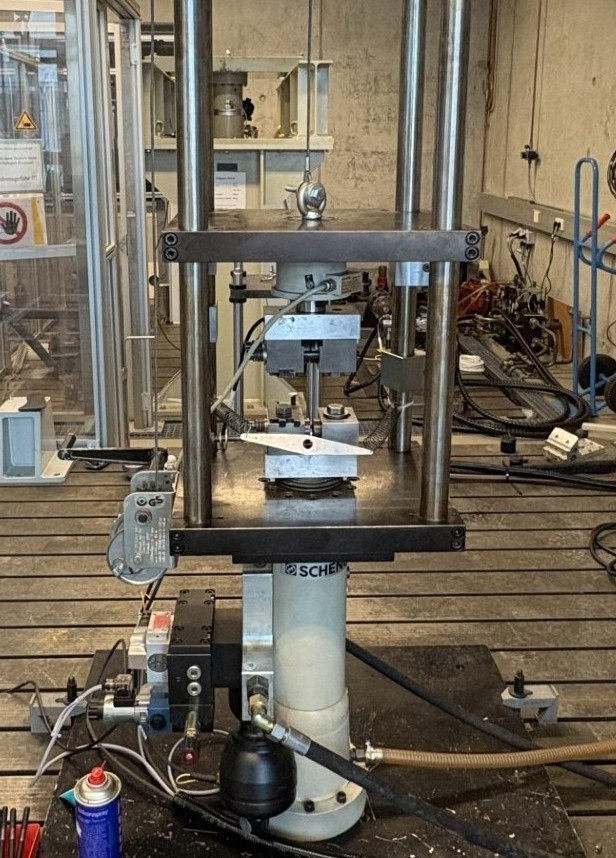
\includegraphics[width=\textwidth]{Hydropulsanlage_gesamt}
        \end{minipage}%
    }
    
    \vspace{0.5cm} % Erzeugt einen sauberen vertikalen Abstand zwischen den beiden Elementen

    % --- UNTERES TEILBILD (DIAGRAMM) ---
    \subfloat[Schematischer Aufbau und signaltechnischer Regelkreis\label{fig:Regelkreis_Schema}]{%
        \begin{minipage}{1.0\textwidth} % Nutzt die volle Textbreite für maximale Lesbarkeit
            \centering
            \begin{tikzpicture}[
                >=latex, 
                scale=1.0, every node/.style={scale=0.85}, % Skalierung leicht erhöht für die volle Breite
                font=\sffamily\small, 
                block/.style={rectangle, draw, minimum width=2.5cm, minimum height=0.9cm, align=center, fill=white, thick},
                sensor/.style={diamond, draw, minimum width=0.9cm, minimum height=0.9cm, fill=white, thick},
                line/.style={draw, ->, thick},
                signal/.style={draw, ->, dashed, thick}
            ]
            
                % --- PRÜFSTAND (LINKS) ---
                \draw[thick] (0,0) rectangle (1.6,3);
                \draw[thick, fill=white] (0,1.4) rectangle (1.6,1.6); 
                \draw[ultra thick] (0.8,-0.9) -- (0.8,1.4); 
                \draw[ultra thick] (0.8,1.6) -- (0.8,4); 
                \node[left=0.3cm] at (0,1.5) {Zylinder};
                \fill[pattern=north east lines] (-0.3,-0.2) rectangle (1.9,0);
                \draw[thick] (-0.3,0) -- (1.9,0);
                \draw[thick, fill=gray!20] (0.65,4.3) rectangle (0.95,5.7);
                \node[right=0.3cm] at (0.95,5) {Probe};
                \draw[thick, fill=white] (0.4,4) rectangle (1.2,4.3);
                \draw[thick, fill=white] (0.4,5.7) rectangle (1.2,6);
                \node[sensor] (loadcell) at (0.8,6.5) {};
                \node[left=0.1cm] at (loadcell.west) {Kraftaufnehmer};
                \draw[thick] (0.8,6) -- (0.8,6.1);
                \node[block, minimum width=0.8cm, minimum height=0.6cm, fill=white] (lvdt) at (0.8,-0.9) {};
                \node[right=1.0cm] at (lvdt.west) {Wegaufnehmer};
            
                % --- REGELUNG (RECHTS) ---
                \node[block] (amp) at (6.0, 6.5) {Verstärker};
                \node[block] (scope) at (9.4, 6.5) {Anzeige};
                \node[block] (controller) at (6.0, 4.5) {Regler};
                \node[block] (input) at (9.4, 4.5) {Sollwert};
                \node[block] (valve) at (6.0, 2) {Ventil};
                \node[draw, circle, thick, minimum size=1.0cm] (pump) at (6.0, 0.3) {P};
                \node[right=0.4cm] at (pump) {Aggregat};
            
                % --- VERBINDUNGEN ---
                \draw[line] ([xshift=-0.15cm]pump.north) -- ([xshift=-0.15cm]valve.south); 
                \draw[line] ([xshift=0.15cm]valve.south) -- ([xshift=0.15cm]pump.north);
                \draw[line] ([yshift=0.25cm]valve.west) -- ++(-0.5,0) |- (1.6,2.6); 
                \draw[line] (1.6,2.4) -- ++(0.7,0) |- ([yshift=0.1cm]valve.west);   
                \draw[line] ([yshift=-0.25cm]valve.west) -- ++(-0.5,0) |- (1.6,0.4); 
                \draw[line] (1.6,0.6) -- ++(0.7,0) |- ([yshift=-0.1cm]valve.west);   
                \draw[signal] (loadcell.east) -- (amp.west);
                \draw[signal, ->] (lvdt.west) -- (-2.2,-0.9) |- (6.0,7.5) -- (amp.north);
                \draw[signal] (amp.east) -- (scope.west);
                \draw[signal] (amp.south) -- (controller.north);
                \draw[signal] (input.west) -- (controller.east);
                \draw[signal] (controller.south) -- (valve.north);
                \fill[pattern=north east lines] (-0.5,6.9) rectangle (1.9,7.1);
                \draw[thick] (-0.5,6.9) -- (1.9,6.9);
            
            \end{tikzpicture}
        \end{minipage}%
    }

    % --- GEMEINSAME HAUPTBILDUNTERSCHRIFT ---
    \caption{Servohydraulische Prüfmaschine (Hydropulsanlage) im\protect\\ Maschinendynamik-Labor der OTH: a) Foto-Versuchsaufbau,\protect\\ b) Schematischer Aufbau und Regelkreis\protect\\ (eigene Darstellung in Anlehnung an \cite[Seite 261]{Ölhydraulik2020}).}
    \label{fig:Regelkreis_Hydropulser_Gesamt}
\end{figure}

Die vorhandenen Sensoren zur Regelung der Anlage im Maschinendynamik-Labor sind ein Kraftaufnehmer und ein Wegaufnehmer. Beide können zur Regelung der Anlage verwendet werden. Entsprechend der DIN 50100 wird für den vorliegenden Versuch die Kraftregelung angewendet.
Dabei wird die aktuelle Kraft mittels einer Kraftmessdose aufgenommen. Dieses Ist-Signal wird dann gemäß dem Regelkreislauf in \Figref{fig:Regelkreis_Hydropulser_Gesamt} b) verstärkt und an einen PID-Regler übermittelt, der die Regeldifferenz zwischen dem Ist-Wert und dem Soll-Wert berechnet und in Form eines Stellsignals an das Servoventil weitergibt. Das Signal des Verstärkers kann zusätzlich durch eine Anzeige sichtbar gemacht werden \cite[Seite 262]{Ölhydraulik2020}.

Der Grund für die Anwendung der Kraftregelung besteht darin, dass die Kraftamplitude bei dem Wöhlerversuch konstant gehalten werden soll. Würde die Messung weggeregelt erfolgen, würde sich die Kraft durch den Rissfortschritt und die damit einhergehende Entfestigung des Bauteils kontinuirlich verringern, wodurch die Versuchsergebnisse verfälscht wären \cite[Seite 9]{DIN50100}. 

Im Maschinendynamik-Labor der OTH stehen drei verschiedene Hydropulser zur Verfügung. Für den Schwingfestigkeitsversuch wird der Hydropulser, dessen Zylinder eine Maximalkraft von 16\,kN aufbringen kann, verwendet \cite{oth}. Die gewählte Prüffrequenz liegt bei 40\,Hz. Zur Gewährleistung der Sicherheit kann ein Abbruchkriterium für den Kraft- oder Wegsensor eingestellt werden. Dieses greift bei Kraftabfall oder Hubüberschreitung und schaltet die Anlage ab. 

	
	\subsection{Statistische Auswertung anhand der Norm}
	Als Grundlage der Wöhlerlinie dienen Stichproben, die aus einer Grundgesamtheit, hier allen produzierten Bauteilen, entnommen werden. Der Vorteil von Stichproben liegt beispielsweise in der schnelleren Auswertbarkeit, da sie einen deutlich geringeren Umfang als die Grundgesamtheit aufweisen und dadurch auch Kosten einsparen. Folglich muss die Auswertung mit MATLAB statistisch erfolgen \cite[Seite 20-21]{StatHedderich2020}. 
	
Die Auswertung der Wöhlerlinie folgt einer logarithmischen Normalverteilung. 
\textbf{Eine logarithmische Normalverteilung liegt vor, wenn die Logarithmen einer Größe normalverteilt sind. Im Wöhlerversuch wird angenommen, dass die logarithmierten Schwingspielzahlen einer Normalverteilung folgen. Dadurch können Mittelwert, Standardabweichung und Ausfallwahrscheinlichkeiten statistisch bestimmt werden.\\
Beim Perlenschnurverfahren wird davon ausgegangen, dass die Schwingspielzahlen einer logarithmischen Normalverteilung folgen. Dies bedeutet, dass nicht die Schwingspielzahlen $N$ selbst normalverteilt sind, sondern ihre dekadischen Logarithmen $\lg N$. Durch diese Annahme können die statistischen Kenngrößen der Grundgesamtheit bestimmt werden. Ziel des Verfahrens ist die möglichst genaue Schätzung des Mittelwertes der logarithmierten Schwingspielzahlen $N_{50\,\%,GG}$ sowie der Standardabweichung $s_{\lg N,GG}$. Diese Kenngrößen bilden die Grundlage für die Beschreibung der Streuung der Versuchsergebnisse und ermöglichen die Bestimmung von Ausfallwahrscheinlichkeiten sowie die Berechnung von Wöhlerlinien mit unterschiedlichen Überlebens- bzw. Ausfallwahrscheinlichkeiten. (Tabelle 2,3 und 4)}
	 
Die Wöhlerkurve kann nach zwei unterschiedlichen Prinzipien aufgestellt werden. Entweder wird für alle Proben ein konstantes Spannungsverhältnis R oder eine konstante Mittelspannung $\sigma_m$ eingestellt. Die Spannungsamplitude wird dabei für jede Probe unterschiedlich gewählt, jedoch wird sie während der Versuchsdurchführung konstant gehalten. Als Ergebnis folgt entweder eine Bruchschwingspielzahl $N_B$ oder eine Grenzschwingspielzahl $N_G$. Bei einer Bruchschwingspielzahl werden alle Schwingspiele bis zum Bruch aufgezeichnet. Bei der Grenzschwingspielzahl wird der Versuch beendet und das Versuchsergebnis wird als Durchläufer bezeichnet. Den Zusammenhang zwischen Lebensdauer und Amplitude veranschaulicht \Figref{fig:Schwingungen der Einzelproben}. Probe 1 und 2 versagen aufgrund ihrer großen Amplituden $\sigma_{\text{a1}}$ und $\sigma_{\text{a2}}$ nach ihrer entsprechenden Schwingspielzahl $N_{\text{B1}}$ bzw. $N_{\text{B2}}$ . Der letzte Prüfkörper~n hingegen wird als Durchläufer gewertet, denn aufgrund der verhältnismäßig kleinen Amplitude $\sigma_{\text{an}}$ erfährt dieser kein Versagen \cite[Seite 272]{Werkstofftechnik-Praktikum2021}. 

\begin{figure}[H]
    \centering
\begin{tikzpicture}[
    >=stealth, 
    font=\sffamily\small,
    axis break/.style={
        draw=white, fill=white, postaction={draw=black, decoration={zigzag, segment length=3.5pt, amplitude=2.5pt}, decorate}
    }, >=latex
]
\usetikzlibrary{decorations.pathmorphing}

% --- PARAMETER ---
\def\sigm{1.1}      
\def\gapstart{1.5}  % Ende vor dem gestrichelten Teil
\def\markstart{1.9} % Start der durchgezogenen Linie nach dem Zeitsprung
\def\zackpos{1.7}   % NEUE Position für das Zick-Zack (mittig unter dem gestrichelten Teil)

% --- PROBE 1 ---
\begin{scope}[shift={(0,7.5)}]
    \node[anchor=west] at (0.2,2.5) {Probe 1};
    \draw[thick, ->] (0,0) -- (7.5,0) node[below left] {Zeit $t$};
    \draw[thick, ->] (0,-0.2) -- (0,2.5) node[rotate=90, left, at start, xshift=2.3cm, yshift=0.95cm] {Spannung $\sigma$};
    
    % ZICK-ZACK NACH LINKS VERSCHOBEN (unter gestrichelten Teil)
    \draw (\zackpos-0.1, -0.12) -- (\zackpos-0.1, 0.12); 
    \draw (\zackpos+0.1, -0.12) -- (\zackpos+0.1, 0.12);
    \draw[axis break] (\zackpos-0.1, 0) -- (\zackpos+0.1, 0);

    \draw[dashed] (0,\sigm) -- (5.0,\sigm) node[left, pos=0.01] {$\sigma_m$};
    \draw (0, 2.1) -- (4.17, 2.1); 

    \draw[thick] plot[domain=0:\gapstart, samples=80] (\x, {\sigm + 1.0*sin(\x*360*1.5)});
    \draw[thick, dashed] plot[domain=\gapstart:\markstart, samples=30] (\x, {\sigm + 1.0*sin(\x*360*1.5)});
    \draw[thick] plot[domain=\markstart:4.17, samples=100] (\x, {\sigm + 1.0*sin(\x*360*1.5)});

    \draw[dashed] (4.17, 2.1) -- (4.17, 0) node[below] {$N_{B1}$};
    \filldraw[fill=white] (4.17, 2.1) circle (1.5pt) coordinate (P1);
    \node[right] at (4.87, 2.4) {Bruch};
    \draw[thin] (P1) -- (4.77, 2.4); 
    \draw[<->] (4.47, \sigm) -- (4.47, 2.1) node[midway, right] {$\sigma_{a1}$};
    \draw (4.17, 2.1) -- (4.87, 2.1);
\end{scope}

% --- PROBE 2 ---
\begin{scope}[shift={(0,3.75)}]
    \node[anchor=west] at (0.2,2.3) {Probe 2};
    \draw[thick, ->] (0,0) -- (7.5,0) node[below left] {Zeit $t$};
    \draw[thick, ->] (0,-0.2) -- (0,2.5) node[rotate=90, left, at start, xshift=2.3cm, yshift=0.95cm] {Spannung $\sigma$};
    
    \draw (\zackpos-0.1, -0.12) -- (\zackpos-0.1, 0.12); 
    \draw (\zackpos+0.1, -0.12) -- (\zackpos+0.1, 0.12);
    \draw[axis break] (\zackpos-0.1, 0) -- (\zackpos+0.1, 0);

    % Mittellinie korrigiert
    \draw[dashed] (0,\sigm) -- (6.0,\sigm) node[left, pos=0.01] {$\sigma_m$};
    \draw (0, 1.8) -- (5.5, 1.8); 

    \draw[thick] plot[domain=0:\gapstart, samples=80] (\x, {\sigm + 0.7*sin(\x*360*1.5)});
    \draw[thick, dashed] plot[domain=\gapstart:\markstart, samples=30] (\x, {\sigm + 0.7*sin(\x*360*1.5)});
    \draw[thick] plot[domain=\markstart:5.5, samples=150] (\x, {\sigm + 0.7*sin(\x*360*1.5)});

    \draw[dashed] (5.5, 1.8) -- (5.5, 0) node[below] {$N_{B2}$};
    \filldraw[fill=white] (5.5, 1.8) circle (1.5pt) coordinate (P2);
    \node[right] at (6.2, 2.1) {Bruch};
    \draw[thin] (P2) -- (6.1, 2.1);
    \draw[<->] (5.8, \sigm) -- (5.8, 1.8) node[midway, right] {$\sigma_{a2} < \sigma_{a1}$};
    \draw (5.5, 1.8) -- (6.2, 1.8);
\end{scope}

% --- PROBE n (Schwingung endet auf Mittellinie) ---
\begin{scope}[shift={(0,0)}]
    \node[anchor=west] at (0.2,2.2) {Probe $n$};
    
    \draw[thick, ->] (0,0) -- (8.0,0) node[below left] {Zeit $t$};
    \draw[thick, ->] (0,-0.2) -- (0,2.5) node[rotate=90, left, at start, xshift=2.3cm, yshift=0.95cm] {Spannung $\sigma$};
    
    \draw (\zackpos-0.1, -0.12) -- (\zackpos-0.1, 0.12); 
    \draw (\zackpos+0.1, -0.12) -- (\zackpos+0.1, 0.12);
    \draw[axis break] (\zackpos-0.1, 0) -- (\zackpos+0.1, 0);

    \draw[dashed] (0,\sigm) -- (7.33,\sigm) node[left, pos=0] {$\sigma_m$};
    \draw (0, 1.5) -- (7.33, 1.5);

    % Schwingung endet exakt bei 7.33 (Schnittpunkt mit Mittellinie)
    \draw[thick] plot[domain=0:\gapstart, samples=80] (\x, {\sigm + 0.4*sin(\x*360*1.5)});
    \draw[thick, dashed] plot[domain=\gapstart:\markstart, samples=30] (\x, {\sigm + 0.4*sin(\x*360*1.5)});
    \draw[thick] plot[domain=\markstart:7.33, samples=200] (\x, {\sigm + 0.4*sin(\x*360*1.5)});

    \node[anchor=south] at (6.6, 1.6) {\underline{kein Bruch}};
    
    % DAUERFESTIGKEITSPFEIL: Setzt exakt bei 7.33 auf der Mittellinie an
    \draw[ultra thick, ->] (7.33, \sigm) -- (8.1, \sigm) node[right, yshift=-3pt] {$\infty$};
   
    \draw (7.33, 1.5) -- (7.9, 1.5); 
    \draw[<->] (7.5, \sigm) -- (7.5, 1.5) node[midway, right] {$\sigma_{an} < \sigma_{an-1}$};
\end{scope}
\end{tikzpicture}
\caption{Schwingungen der Einzelproben mit gleicher Mittelspannung und unterschiedlicher Spannungsamplitude (In Anlehnung an \cite[Seite 273]{Werkstofftechnik-Praktikum2021}).}
\label{fig:Schwingungen der Einzelproben}
\end{figure}

Zur Ableitung der Wöhlerlinie aus den experimentell ermittelten Schwingspielzahlen der einzelnen Proben, wird die eingestellte Spannungsamplitude $\sigma_a$ über die erreichte Schwingspielzahl $N$ doppelt logarithmisch aufgetragen. Folglich werden die Datenpunkte der in \Figref{fig:Schwingungen der Einzelproben} abgebildeten Proben 1 und 2 in  \Figref{fig:Wöhlerkurve} eingetragen. Dies sind die Schnittpunkte der jeweiligen Spannungsamplituden $\sigma_{\text{a1}}$ und $\sigma_{\text{a2}}$ mit den beiden Bruchschwingspielzahlen $N_{\text{B1}}$ und  $N_{\text{B2}}$, verteilt in einem Streuband (\Figref{fig:Wöhlerkurve} (Nummer 2)).
Aus den Versuchsergebnissen mehrerer Proben ensteht nach statistischer Auswertung eine wie in \Figref{fig:Wöhlerkurve} gezeigte Kurve. Die Wöhlerkurve wird nach DIN 50100 in den Bereich der Kurzzeitfestigkeit (LCF, engl. Low Cycle Fatigue), der Zeitfestigkeit (HCF, engl. High Cycle Fatigue) und der Langzeitfestigkeit (LLF, engl. Long Life Fatigue) eingeteilt  \cite[Seite 17]{DIN50100}. In der Praxis zeigt sich, dass in den Bereichen der Zeitfestigkeit und der Langzeitfestigkeit die Proben eine signifikante statistische Streuung aufweisen. Ursache hierfür sind eine Vielzahl von Einflussfaktoren, wie beispielsweise Werkstoffinhomogenitäten oder eine ungleiche Einspannung, deren Wirkungen das Verhalten der Probe beeinflussen \cite[Seite 259]{Laepple2016}.

\begin{figure}[H]
    \centering
\begin{tikzpicture}[
    scale=1.1, 
    font=\sffamily\small,
    >=stealth
]

% --- RAHMEN ---
\draw[thick] (0,0) -- (8,0) -- (8,7) -- (0,7) -- cycle; 

% --- VERTIKALE ACHSE ---
\draw[thick, ->] (0,0) -- (0,7.8) node[above] {$\sigma_a$ (lg)};

% --- LOG-SKALA (Oben & Unten) ---
\foreach \expo in {0,1,2,3,4,5,6,7} {
  \draw[thick] (\expo,0) -- (\expo,0.25); \draw[thick] (\expo,7) -- (\expo,6.75); 
  \foreach \sub in {2,3,4,5,6,7,8,9} {
    \pgfmathsetmacro{\tickx}{\expo + log10(\sub)}
    \ifdim \tickx pt < 8.01pt
      \draw[thin] (\tickx,0) -- (\tickx,0.1); \draw[thin] (\tickx,7) -- (\tickx,6.9);
    \fi
  }
}
\draw[thick] (8,0) -- (8,0.25); \draw[thick] (8,7) -- (8,6.75);

% Achsbeschriftungen unten
\foreach \x/\l in {0/10^0, 2/10^2, 4/10^4, 6/10^6, 8/10^8} \node[below=4pt] at (\x,0) {$\l$};
\node[below left] at (9.6,0) {$N$ (lg)};
\draw[thick, ->] (8,0) -- (9.0,0);

% --- PARAMETER ---
\def\nkpos{6.5}
\def\ngpos{7.2}
\def\h_nk{1.8} 

% --- STREUBAND (Graue Fläche 2) ---
\fill[gray!20] 
    (0,6.0) to[out=-2, in=165] (3.8,5.2) -- (\nkpos,1.2) -- (8,1.1) -- 
    (8,2.2) -- (\ngpos,2.2) -- (4.2,5.8) to[out=178, in=-2] (0,6.2) -- cycle;

\draw[thin] (0,6.0) to[out=-2, in=165] (3.8,5.2) -- (\nkpos,1.2) -- (8,1.1);
\draw[thin] (0,6.2) to[out=-2, in=178] (4.2,5.8) -- (\ngpos,2.2) -- (8,2.2);

% --- 1 - ZEITFESTIGKEIT & FETTER ÜBERGANG ---
\draw[ultra thick] (4.5, 5.0) -- (\nkpos, \h_nk); 
\draw[ultra thick] (\nkpos, \h_nk) -- (\ngpos, \h_nk); 

% --- PUNKTE (3) UND HILFSLINIEN ---
% Punkt 1 (unverändert oben): (4.7, 4.8)
\draw[dashed, thin, gray] (4.7, 4.8) -- (0, 4.8) node[left, black] {$\sigma_{a1}$};
\draw[dashed, thin, gray] (4.7, 4.8) -- (4.7, 0) node[below=15pt, black] {$N_{B1}$};

% Punkt 2 (jetzt weiter unten/rechts): (5.6, 3.4)
\draw[dashed, thin, gray] (5.6, 3.4) -- (0, 3.4) node[left, black] {$\sigma_{a2}$};
\draw[dashed, thin, gray] (5.6, 3.4) -- (5.6, 0) node[below=15pt, black] {$N_{B2}$};

% Alle Punkte zeichnen (gefüllt)
\foreach \p in {(4.7, 4.8), (4.5, 4.75), (5.0, 4.5), (4.9, 4.2), (5.3, 3.9), (5.6, 3.4), (6.1, 3.1), (5.7, 2.7), (6.2, 2.5), (6.3, 1.85)} {
    \fill \p circle (2pt);
}


% --- 4 - DURCHLÄUFER ---
\foreach \y in {1.8, 1.6, 1.4} {
    \draw (\ngpos, \y) circle (2pt);
    \draw[->] (\ngpos, \y) -- (7.8, \y);
}

% --- HINWEISSTRICHE (Optimiert nach deiner Skizze) ---
% 1: Zeitfestigkeitsgerade
\node (n1) at (4.2, 3.4) {1};
\draw[->, thin] (n1) -- (5.2, 3.9);

% 2: Streuband (zeigt auf die obere Begrenzungslinie)
\node (n2) at (6.4, 5.4) {2};
\draw[->, thin] (n2) -- (5.1, 4.7);

% 3: Ausfall (zeigt auf die Punktegruppe)
\node (n3) at (7.0, 3.7) {3};
\draw[->, thin] (n3) -- (6.15, 3.15);

% 4: Durchläufer (zeigt auf den Knickpunkt NG)
\node (n4) at (7.7, 2.4) {4};
\draw[->, thin] (n4) -- (\ngpos, 1.9);

% 5: Statische Festigkeit (zeigt auf den Kurvenbeginn links)
\node (n5) at (-0.6, 6.6) {5};
\draw[->, thin] (n5) -- (0, 6.05);

% --- TRENNLINIEN ---
% --- TRENNLINIEN ---
\draw[thin] (4,0) -- (4,7.0); % Bleibt: LCF/HCF Grenze

% Ändere \ngpos zu \nkpos für die durchgehende Linie:
\draw[thin] (\nkpos,0) -- (\nkpos,7.0); 

% Falls du NG nur als kurzen Strich bis zum Streuband willst:
\draw[thin] (\ngpos,0) -- (\ngpos,1.6); 
\node[below=16pt] at (\nkpos,0) {$N_K$};
\node[below=16pt] at (\ngpos,0) {$N_G$};

% --- BEREICHE OBEN ---
\draw[<->] (0,7.3) -- (4,7.3) node[midway, above, align=center] {Kurzzeit-\\festigkeit (LCF)};
\draw[<->] (4,7.3) -- (\nkpos,7.3) node[midway, above, align=center] {Zeit-\\festigkeit (HCF)}; % Ende jetzt bei NK
\draw[<->] (\nkpos,7.3) -- (8,7.3) node[midway, above, align=center] {Langzeit-\\ festigkeit\\ (LLF)}; % Start jetzt bei NK

% Horizontale Referenzlinie
\draw[thin] (0,\h_nk) -- (\nkpos,\h_nk) node[left, pos=0] {$L_{al, 1E7}$};

\end{tikzpicture}

% --- LEGENDE (als Text unter der Abbildung) ---
\vspace{0.5cm}
\begin{flushleft}
\textbf{Legende}\\
1 Zeitfestigkeitsgerade\\
2 Streuband der Versuche\\
3 Ausfall\\
4 Durchläufer\\
5 Statische Festigkeit
\end{flushleft}
\caption{Prinzipskizze einer Wöhlerkurve (In Anlehnung an \cite[Seite 17]{DIN50100}).}
\label{fig:Wöhlerkurve}
\end{figure}

Die statische Festigkeit wird durch Pfeil 5 in \Figref{fig:Wöhlerkurve} repräsentiert und stellt die maximal ertragbare statische Belastung dar. Nummer 3 kennzeichnet eine Probe im Zeitfestigkeitsbereich. Da sie eines der beiden Ausfallkriterien (Anriss oder Bruch) erreicht hat, wird sie als Ausfallprobe bezeichnet. Nummer 4 hingegen liegt im Bereich der Langzeitfestigkeit und wird als Durchläufer gewertet, da die Grenzschwingspielzahl $N_G$ erreicht ist.

Die großen Amplituden im Bereich der Kurzzeitfestigkeit bewirken eine geringe Lebensdauer. Dabei liegen die Messergebnisse zwischen \(10^{0}\) und \(10^{4}\) Schwingspielen. Gemäß der DIN 50100 wird der Kurzzeitfestigkeitsbereich (LCF) nicht betrachtet, da dort ein dehnungs- und schiebungskontrollierter Versuch erfolgen muss. Die Zeitfestigkeit liegt zwischen  \(10^{4}\) Schwingspielen und der Knickschwingspielzahl $N_K$ und wird durch die Zeitfestigkeitsgerade (siehe Nummer 1 in \Figref{fig:Wöhlerkurve}) beschrieben.

Am Ende der Zeitfestigkeitsgerade folgt die Knickschwingspielzahl. Diese liegt im Bereich zwischen $5 \cdot 10^5$ und $10^7$ Lastwechseln und repräsentiert den Übergang von der Zeitfestigkeit zur Langzeitfestigkeit.
Zum Bereich der Langzeitfestigkeit zählen alle Schwingspiele, die größer sind als die Knickschwingspielzahl $N_K$ \cite[Seite 9-17]{DIN50100}.

Die DIN 50100 unterscheidet drei Typen der Langzeitfestigkeit, die einen unterschiedlichen Verlauf der Wöhlerkurve nach dem Knickpunkt darstellen:

% Im Dokument:
\begin{itemize}
    \item {Typ I: horizontaler Verlauf}
    \item {Typ II: Gerade mit geringerer Steigung $k^*$}
  \item {Typ III: zuerst horizontaler Verlauf und dann noch weiterer Abfall der Kurve}
\end{itemize}
  
  Da Typ III in der Norm außdrücklich nicht behandelt wird, veranschaulicht \Figref{fig:Vergleich Typ I und Typ II der Wöhlerkurve} nur den Vergleich zwischen Typ I und II. 

  
\begin{figure}[H]
    \centering
    \sffamily\small
    
    \begin{tikzpicture}[scale=1.1, >=stealth]
        % Achsen
        \draw[thick, ->] (0,0) -- (11,0) node[below left=0.1cm, xshift=2.5cm] {Schwingspielzahl $N$ (log)};
        \draw[thick, ->] (0,0) -- (0,5.5) node[midway, left=0.6cm, rotate=90, xshift=90pt] {Spannungsamplitude $\sigma_a$ (log)};

        % --- Wöhlerkurve Typ I ---
        \draw[thick] (0.2, 4.5) 
            .. controls (2.5, 4.5) and (3.5, 1.4) .. (5.5, 1.4) 
            -- (10.5, 1.4); 

        % Steigungsdreieck k (hängt unter Kurve I im Zeitfestigkeitsbereich)
        % Horizontale oben, vertikale geht nach unten zur Kurve
        \draw[thin, gray] (1.7, 3.35) -- (1.7, 2.6) -- (2.6, 2.6);
        \node[below left, scale=0.8] at (1.6, 3.1) {$k$};

        % --- Wöhlerkurve Typ II ---
        \draw[thick, dashed] (0.8, 3.8) 
            .. controls (2.2, 3.5) and (3.5, 1.2) .. (4.8, 1.0) 
            -- (10.5, 0.45); 

        % Steigungsdreieck k* (hängt unter Kurve II im Auslauf)
        \draw[thin, gray] (7.7, 0.7) -- (6.0, 0.7) -- (6.0, 0.9);
        \node[below, scale=0.8] at (6.0, 0.7) {$k^*$};

        % Vertikale Hilfslinien NG
        \draw[thin] (5.5, 1.4) -- (5.5, 0);
        \node[below=0.6cm, scale=0.85] at (5.5, 0) {$N_G = 5 \cdot 10^6$};

        \draw[thin] (8.5, 0.6) -- (8.5, 0);
        \node[below=0.6cm, scale=0.85] at (8.5, 0) {$N_G = 10^7$ bis $10^8$};

        % Pfeile für sigma_aL
        \draw[<->] (5.5, 0.05) -- (5.5, 1.35) node[midway, left, scale=0.8] {$\sigma_{aL}$};
        \draw[<->] (8.5, 0.05) -- (8.5, 0.55) node[midway, left, scale=0.8] {$\sigma_{aL}$};

        % Legende
        \begin{scope}[shift={(6.2, 4.8)}]
            \draw[thick] (0, 0) -- (0.8, 0) node[right] {Wöhlerkurve -- Typ I};
            \node[right, scale=0.85] at (0.8, -0.3) {$\rightarrow$ krz-Stähle};
            
            \draw[thick, dashed] (0, -1.0) -- (0.8, -1.0) node[right] {Wöhlerkurve -- Typ II};
            \node[right, align=left, scale=0.85] at (0.8, -1.7) {
                $\rightarrow$ kfz-Stähle\\
                $\rightarrow$ hdp-Metalle\\
            };
        \end{scope}

    \end{tikzpicture}
    \caption{Vergleich Typ I und Typ II der Wöhlerkurve.}
    \label{fig:Vergleich Typ I und Typ II der Wöhlerkurve}
\end{figure}


Zu erkennen ist, dass bei Typ II die Spannungsamplitude weiter abfällt, jedoch mit einer geringeren Steigung $k^*$. Im Unterschied dazu verläuft Typ I horizontal ab der Grenzschwingspielzahl $N_G$. 

\clearpage

	\subsection{Experimentelle Verfahren zur Bestimmung der Zeitfestigkeit}
Zur Bestimmung der Lage der Zeitfestigkeit können laut DIN 50100 zwei Verfahren angewendet werden, die zur Versuchsdurchführung dienen. Im Bereich der Zeitfestigkeit tritt immer ein Ausfall der Probe ein.

Beim sogenannten Horizontenverfahren werden zwei Lasthorizonte gewählt, die möglichst nah an den Grenzen des Kurzzeit- und des Langzeitfestigkeitbereichs liegen, um dort anschließend mehrere Proben zu prüfen (siehe \Figref{fig:Diagramm_Horizontenverfahren}).

\begin{figure}[H]
    \centering
    \begin{tikzpicture}[>=stealth, thick]
% Achsen
\draw[->, line width=1.2pt] (0,0) -- (9,0)
    node[below right] {$N\,(\lg)$};

\draw[->, line width=1.2pt] (0,0) -- (0,6.3)
    node[above left, rotate=90] {$\sigma_a\,(\lg)$};

% Horizontale Linien
\draw[dashed] (0,4.5) -- (8.1,4.5);
\draw[dashed] (0,1.8) -- (8.1,1.8);

% Beschriftungen links
\node[left] at (0,4.5) {$S_{a1}$};
\node[left] at (0,1.8) {$S_{a2}$};

% 50%-Wöhlerlinie, oben weiter links durch Punktbereich
\draw[line width=1.6pt] (1.2,5.2) -- (6.7,0.8);

% Beschriftung gerade
\node at (5.3,3.6) {50\,\%-Wöhlerlinie};

% Obere rote Punkte
\foreach \x in {0.7,1.3,1.7,2.0,2.3,2.6,3.2}
{
    \fill[black] (\x,4.5) circle (2.5pt);
}

% Untere rote Punkte
\foreach \x in {3.8,4.6,5.1,5.5,5.8,6.3,6.9,7.8}
{
    \fill[black] (\x,1.8) circle (2.5pt);
}

\end{tikzpicture}
        \caption{Horizontenverfahren \cite[Seite 26]{Dissertation_Woehler}.}
        \label{fig:Diagramm_Horizontenverfahren}
\end{figure}

Der Nachteil dieses Verfahrens besteht darin, dass es nur dann verwendet werden kann, wenn die Lage der Kurz- und Langzeitfestigkeitsintervalle bekannt ist \cite[Seite 273]{Eulitz2022}. 

Das Perlenschnurverfahren wird immer dann herangezogen, wenn die Grenzen des Zeitfestigkeitsbereichs noch nicht exakt verifiziert wurden. Ein weiterer entscheidender Vorteil äußert sich dadurch, dass auch bei einer geringen Probenanzahl eine geeignete Wöhlerlinie bestimmt werden kann. Die Vorgehensweise ist ein stufenweises Adaptieren der unterschiedlichen Lasthorizonte bis zu den Übergängen der Kurz- und Langzeitfestigkeit. Es ist zudem möglich, mehrere Proben auf einem Lasthorizont zu prüfen \cite[Seite 278]{Eulitz2022}. 

Hierbei sind jedoch zwei wesentliche Einschränkungen zu berücksichtigen. Sowohl bei einer zu geringen Probenzahl (n < 10 Proben) als auch bei einem zu geringen Quotienten der Schwingspielzahl des obersten und des untersten Lasthorizonts (Quotient < 5) verlieren sämtliche zu schätzenden Kenngrößen (Mittelwert, Standardabweichung und Steigung der Zeitfestigkeitsgeraden) ihre Aussagekraft. Diese erlauben dann keine zuverlässigen statistischen Aussage über die Grundgesamtheit. 

Für die Standardabweichung der Grundgesamtheit wird in der DIN 50100 ein Bereich zwischen 0,10 und 0,30 angeraten. Wenn keine Referenzwerte vorliegen, wird eine Standardabweichung der Grundgesamtheit von $s_{\lg N,\text{GG}}$=0,20 empfohlen \cite[Seite 30]{DIN50100}. Mit der noch folgenden \Eqref{eq:S_Perlenschnurverfahren} wird die Standardabweichung der Stichprobe berechnet. Im Idealfall stimmt diese mit der wahren Standardabweichung der Grundgesamtheit überein. Da die tatsächliche Standardabweichung üblicherweise vor dem Versuch nicht bekannt ist, wird die zuvor erwähnte $s_{\lg N,\text{GG}}$=0,20 als initialer Schätzwert herangezogen. Dies ist lediglich ein Erfahrungswert und entspricht nicht zwingend der wahren Standardabweichung der Grundgesamtheit.

\begin{figure}[H]
    \centering
    \begin{tikzpicture}
        % 1. Das bereinigte Bild einbinden und die Dimensionen festlegen
        \node[anchor=south west, inner sep=0] (bild) at (0,0) {
            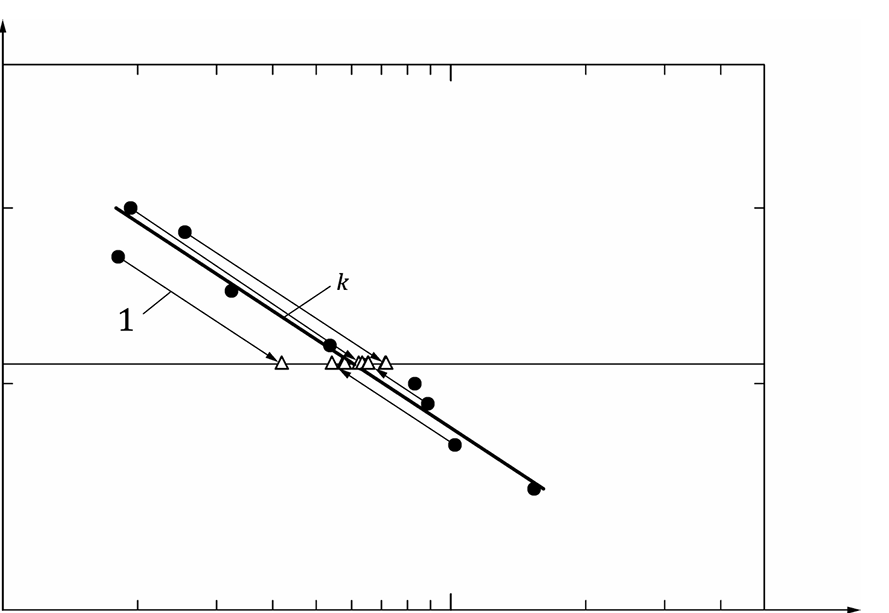
\includegraphics[width=0.8\textwidth]{Perlenschnurverfahren}
        };
        
        % 2. Ein relatives Koordinatensystem (0,0 bis 1,1) über das Bild legen
        \begin{scope}[x={(bild.south east)}, y={(bild.north west)}]
            
            % --- VERTIKALE ACHSE (Y-Achse) ---
            % Beschriftung oben links an der Achse
            \node[anchor=east, font=\small] at (0.0, 0.92) {$\sigma_{\mathrm{a}}\;\mathrm{(lg)}$};
            
            % Fiktiver Lasthorizont (Mitte links)
            \node[anchor=east, font=\small] at (0.0, 0.42) {$\sigma_{\mathrm{a,fiktiv}}$};
            
            
            % --- HORIZONTALE ACHSE (X-Achse) ---
            % Achsentick 10^5
            \node[anchor=north, font=\small] at (0.0, 0.0) {$10^5$};
            
            % Achsentick 10^6
            \node[anchor=north, font=\small] at (0.52, 0.0) {$10^6$};
            
            % Beschriftung unten rechts an der Achse
            \node[anchor=north, font=\small] at (0.93, 0.0) {$N\;\mathrm{(lg)}$};
            
        \end{scope}
    \end{tikzpicture}
    
            \vspace{0.2cm} % Kleiner Abstand zum Bild
        \begin{minipage}{0.75\textwidth}
            \small
            \textbf{Legende:}
            \begin{description}
                \item[1] Verschiebung der Versuchsergebnisse entlang der Geradenneigung
            \end{description}
        \end{minipage}
        \vspace{0.2cm} % Kleiner Abstand zur Caption
        
        \caption{Ermittlung der Standardabweichung Perlenschnurverfahren \cite[Seite 56]{DIN50100}.}
        \label{fig:Diagramm_Perlenschnurverfahren}
\end{figure}


Die hervorgehobene Linie kennzeichnet die 50\%-Zeitfestigkeitsgerade mit der Steigung k. Mit der Nummer 1 ist die verschobene Linie bezeichnet, die die neuen fiktiven Schwingspielzahlen auf dem fiktiven Lasthorizont abbildet. 

Die Zeitfestigkeitsgerade kann mit der sogenannten Basquin-Gleichung (\Eqref{eq:Zeitfestigkeitsgerade_C}) gemäß DIN 50100 ermittelt werden:

\begin{equation}\label{eq:Zeitfestigkeitsgerade_C}
    N = C \cdot \sigma_{\mathrm{a}}^{-k}.
\end{equation}

Die Parameter k und C in \Eqref{eq:Zeitfestigkeitsgerade_C} stehen für die Steigung der Zeitfestigkeitsgeraden und für den Achsenabschnitt der Schwingspielzahl N für $\sigma_a$=1. 
In der noch folgenden Auswertung des Wöhlerversuches wird bei der Erstellung der Wöhlerlinie die Kraftamplitude über die Schwingspielzahl aufgetragen. Die Formeln werden hier nur exemplarisch anhand der Spannungsamplitude erläutert, analog zur Norm. Aus diesem Grund kann auch in \Eqref{eq:Zeitfestigkeitsgerade_C} sowie in den folgenden Gleichungen mit der Kraftamplitude gerechnet werden. 

Nach Anwendung des dekadischen Logarithmus auf \Eqref{eq:Zeitfestigkeitsgerade_C} wird diese wie folgt geschrieben:

    \begin{equation}\label{eq:Zeitfestigkeitsgerade_log}
    \lg N = \lg C - k \cdot \lg \sigma_a.
    \end{equation}
    
\Eqref{eq:Zeitfestigkeitsgerade_log} kann durch Substitution in eine Geradengleichung umgeformt werden (siehe \Eqref{eq:substitution}).

	\begin{equation}
	y = a_0 + a_1 \cdot x
	\label{eq:substitution}
	\end{equation}
	
Die verwendeten substituierten Variablen sind dabei wie folgt definiert:
\begin{align*}
y   &= \lg N   \\
a_0 &= \lg C   \\
a_1 &= -k  \\           
x   &= \lg \sigma_{\text{a}} .
\end{align*} 

Beide Parameter $a_0$ und $a_1$ werden mit der Methode der kleinsten Fehlerquadrate nach \Eqref{eq:reg_a1} und \Eqref{eq:reg_a0} bestimmt. 

\begin{equation}\label{eq:reg_a1}
    a_1 = \frac{n \cdot \sum(x \cdot y) - \sum x \cdot \sum y}{n \cdot \sum(x^2) - (\sum x)^2}
\end{equation}

\begin{equation}\label{eq:reg_a0}
    a_0 = \frac{1}{n} \left( \sum y - a_1 \cdot \sum x \right)
\end{equation}

Mit den bestimmten Regressionsparametern können nun die Steigung $k$ und der Lageparameter $C$ der Basquin-Gleichung in \Eqref{eq:reg_C} und \Eqref{eq:reg_k} bestimmt werden. 

\begin{equation}\label{eq:reg_C}
    C = 10^{a_0}
\end{equation}

\begin{equation}\label{eq:reg_k}
    k = -{a_1}
\end{equation}

Die damit ermittelte Regressionsgerade repräsentiert die 50\%-Wöhlerlinie. Dies impliziert, dass 50\% der Bauteile bei dieser Linie bereits ausgefallen sind. Um die Wöhlerlinie aussagekräftiger anzufertigen, wird eine Linie bei 10\% und eine Linie bei 90\% Ausfallwahrscheinlichkeit ergänzt.  
Unter der Prämisse, dass die Standardabweichung auf allen Lasthorizonten gleich ist (DIN 50100), resultiert, dass die 10$\%$ und 90$\%$ Ausfallwahrscheinlichkeitslinien parallel zur 50$\%$-Linie angetragen werden können. 

Die Standardabweichung wird ermittelt, indem jeder Versuchspunkt auf einen virtuellen Lasthorizont, der frei wählbar ist, verschoben wird (siehe \Figref{fig:Diagramm_Perlenschnurverfahren}). 

 Die entsprechende Formel, die die neue fiktive Schwingspielzahl nach der Verschiebung angibt ist \Eqref{eq:N_fiktiv}.

\begin{equation}\label{eq:N_fiktiv}
    N_{i,\mathrm{fiktiv}} = N_i \cdot \left( \frac{\sigma_{\mathrm{a,fiktiv}}}{\sigma_{\mathrm{a},i}} \right)^{-k}
\end{equation}

Mit \Eqref{eq:mittelwert} wird der Mittelwert der Schwingspielzahlen des fiktiven Lasthorizontes gebildet und anschließend mit \Eqref{eq:rueckrechnung} wieder entlogarithmiert, sodass die Schwingspielzahl der 50\%-Wöhlerlinie folgt. 

\begin{subequations}
\label{eq:gesamte_gleichung}
\begin{align}
\lg N_{50\%,\text{fiktiv}} &= \frac{1}{n} \sum \lg N_{i,\text{fiktiv}} \label{eq:mittelwert} \\[1ex]
\rightarrow \quad N_{50\%,\text{fiktiv}} &= 10^{\lg N_{50\%,\text{fiktiv}}} \label{eq:rueckrechnung}
\end{align}
\end{subequations}

Die Standardabweichung in \Eqref{eq:S_Perlenschnurverfahren} gibt an, wie stark die Versuchsergebnisse um den in \Eqref{eq:rueckrechnung} berechneten Mittelwert des fiktiven Lasthorizonts schwanken. 

\begin{equation}\label{eq:S_Perlenschnurverfahren}
\tilde{s}_{\lg N} = \sqrt{\frac{1}{n - 2} \cdot \sum \left( \lg N_{i,\text{fiktiv}} - \lg N_{50\%,\text{fiktiv}} \right)^2}
\end{equation}


Die DIN 50100 sieht für einen kleinen Stichprobenumfang einen Korrekturfaktor für die Standardabweichung vor (\Eqref{eq:s_korrektur}). 

\begin{equation}\label{eq:s_korrektur}
\tilde{s}_{\lg N,\text{korr}} = \tilde{s}_{\lg N} \cdot \frac{n - 1{,}74}{n - 2}
\end{equation}

Die Schwingspielzahlen der statistischen Streubänder der 10\% und 90\% Ausfallwahrscheinlichkeit auf dem fiktiven Lasthorizont können mit folgenden beiden Gleichungen ermittelt werden:

\begin{subequations}
\begin{align}
N_{90\%} &= 10^{\left( \lg N_{50\%,\text{fiktiv}} + 1{,}282 \cdot \tilde{s}_{\lg N,\text{korr}} \right)} \label{eq:N90} \\[1ex]
N_{10\%} &= 10^{\left( \lg N_{50\%,\text{fiktiv}} - 1{,}282 \cdot \tilde{s}_{\lg N,\text{korr}} \right)} \label{eq:N10}
\end{align}
\end{subequations}

Die ermittelte Zeitfestigkeitsgerade kann nun in die sich ergebenden Punkte der Schwingspielzahl $N_\text{90\%}$ und $N_\text{10\%}$ verschoben werden. 

Einbezogen werden dürfen in die Zeitfestigkeitsgerade alle Messergebnisse deren Lastamplitude über dem höchsten Durchläufer liegt (DIN 50100).

	\subsection{Experimentelle Verfahren zur Bestimmung der Langzeitfestigkeit}
	Zur Bestimmung des Langzeitfestigkeitbereichs werden in der Fachliteratur und in der DIN~50100 verschiedene Verfahren vorgeschlagen. Nachfolgend werden die gängisten Methoden erläutert, um anschließend das geeignetste Verfahren für diese Arbeit auszuwählen:
	\begin{itemize}
    \item Probit Verfahren
    \item Abgrenzungsverfahren
    \item Treppenstufenverfahren nach Hück
	\end{itemize}

Das Probit-Verfahren erfordert eine Festlegung von mindestens vier Lasthorizonten mit gleichem Abstand. Auf jedem Lasthorizont müssen mindestens 10 Proben geprüft werden, um die Streuung auswerten zu können. Jeder Lasthorizont muss dabei mindestens einen Bruch und einen Durchläufer aufweisen. Zu erkennen in \Figref{fig:probit_verfahren} ist, dass die Ausfallwahrscheinlichkeit $P_A$ auf jedem Lasthorizont einzeln ausgewertet wird.  

\begin{figure}[H]
    \centering
    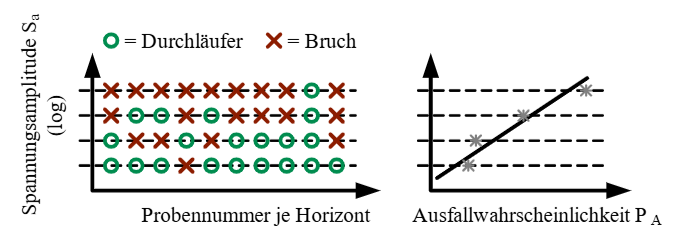
\includegraphics[width=0.75\textwidth]{Probit Verfahren}
    \caption{Probit-Verfahren \cite[Seite 36]{Dissertation_Woehler}.}
    \label{fig:probit_verfahren}
\end{figure}

Das Probit-Verfahren scheidet bei der Auswahl jedoch aus, da mindestens 10 Proben pro Lasthorizont gefordert werden und dadurch im Langzeitfestigkeitsbereich mindestens 40 Proben geprüft werden müssten \cite[Seite 36]{Dissertation_Woehler}. 

Beim Abgrenzungsverfahren wird ähnlich wie beim Horizontenverfahren, auf nur zwei Lasthorizonten geprüft. Die Auswertung erfolgt mittels eines Wahrscheinlichkeitspapieres. 

\begin{figure}[H]
    \centering
    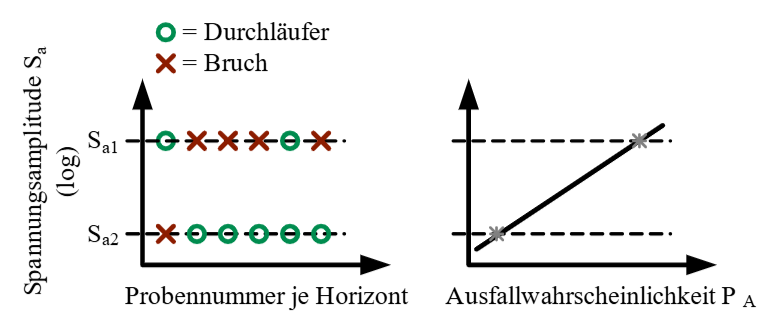
\includegraphics[width=0.75\textwidth]{Abgrenzungsverfahren}
    \caption{Abgrenzungsverfahren \cite[Seite 33]{Dissertation_Woehler}.}
    \label{fig:Abgrenzungsverfahren}
\end{figure}

Das Treppenstufenverfahren prüft auf einem ersten Lasthorizont eine Probe. Ist diese ein Bruch, wird bei der nächsten Probe um eine Stufe mit dem festgelegten Stufensprung reduziert. Ist die Probe hingegen ein Durchläufer, wird bei der nächsten Probe um eine Stufe erhöht. 

Der Hauptgrund, für die Wahl des Treppenstufenverfahrens ist, dass sich mit diesem Verfahren der Mittelwert am besten ermitteln lässt, da sich die Proben um den Mittelwert einpendeln. 

Die Vorgabe für die Laststufen aus der DIN ist es auf ein bis drei Laststufen sowohl Brüche als auch Durchläufer zu haben. Dieser Zustand stellt sich normalerweise ein, wenn der Stufensprung wie folgt gewählt wird: 
\begin{equation}\label{eq:d_lg}
d_{\lg} = 10^{s_{\lg L,\mathrm{GG}}}
\end{equation}

Wenn die Standardabweichung vorab nicht bekannt ist, kann auf empirisch ermittelte Werte zurückgegriffen werden. Folgende \Tabref{tab:Standardabweichung_Treppenstufenverfahren} aus der DIN 50100 beinhaltet für die verschiedenen Materialien die Standardabweichung der Grundgesamtheit und den dazugehörigen Stufensprung $d_{\lg}$:
\begin{table}[h]
\centering
\renewcommand{\arraystretch}{1.5} % Erhöht den Zeilenabstand für bessere Lesbarkeit
\caption{Standardabweichung und Stufensprung Treppenstufenverfahren \cite[Seite 48]{DIN50100}} 
\label{tab:Standardabweichung_Treppenstufenverfahren}
\begin{tabular}{|l|c|c|}
\hline
 & $s_{\lg L,\text{GG}}$ & $d_{\lg}$ \\ \hline
Stahl, spanend bearbeitet & 0,025 & 1,059 \\ \hline
Stahl/Eisen, Gussoberfläche & 0,029 & 1,069 \\ \hline
Stahl, Schweißnaht & 0,038 & 1,091 \\ \hline
Aluminium, Clinchverbindungen & 0,047 & 1,114 \\ \hline
Schrauben & 0,050 & 1,122 \\ \hline
\end{tabular}
\end{table}

Für umfangreichere Werte wird auf die Tabelle im Anhang C der DIN 50100 verwiesen. 

Wenn der Stufensprung ermittelt wurde, können unter ZuHilfenahme einer geschätzten Langzeitfestigkeit $L_{\text{aL},NG}$ die Laststufen anhand von \Eqref{eq:Laststufen} berechnet werden.
\begin{equation} \label{eq:Laststufen} 
    L_i = L_{\text{aL},NG} \cdot (d_{\lg})^i
\end{equation}

Damit Vorversuche die Versuchsergebnisse nicht verfälschen, dürfen diese bei der Versuchsauswertung nicht mit einfließen. Von den Versuchswerten am Anfang fließen nur diejenigen in die Auswertung ein, deren Lastniveau während des Versuches erneut erreicht wurde. So werden beispielsweise in \Figref{fig:Treppenstufenverfahren} die ersten beiden Versuche nicht gewertet. 

\begin{figure}[H]
    \centering
    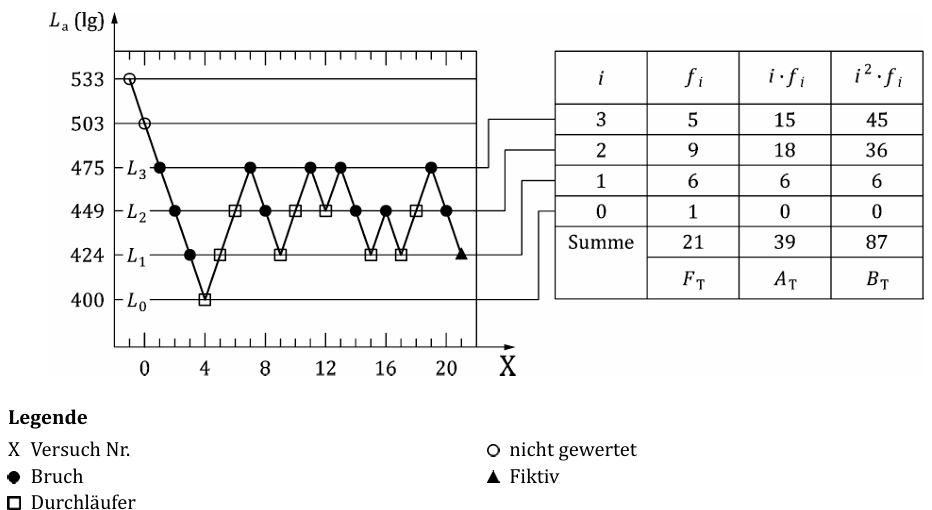
\includegraphics[width=0.9\textwidth]{Treppenstufenverfahren}
    \caption{Treppenstufenverfahren \cite[Seite 60]{DIN50100}}
    \label{fig:Treppenstufenverfahren}
\end{figure}

Ausgehend vom untersten Lasthorizont Null erfolgt die Nummerierung aufsteigend. Die Ereignisse Bruch und Durchläufer werden auf jeder Laststufe einzeln zusammen gezählt und fließen in die drei Hilfsgrößen $F_T$ (\Eqref{eq:F_T}), $A_T$ (\Eqref{eq:A_T}) und $B_T$ (\Eqref{eq:B_T}) zur Berechnung des Mittelwertes ein.

\begin{equation} \label{eq:F_T} 
    F_{\text{T}} = \sum f_i
\end{equation}

\begin{equation} \label{eq:A_T} 
    A_{\text{T}} = \sum i \cdot f_i
\end{equation}

\begin{equation} \label{eq:B_T} 
    B_{\text{T}} = \sum i^2 \cdot f_i
\end{equation}

Der Mittelwert der Langzeitfestigkeit kann dann mit \Eqref{eq:LaL_NG} bestimmt werden.

\begin{equation} \label{eq:LaL_NG} 
    L_{\text{aL},NG} = L_0 \cdot d_{\lg}^{\left(\frac{A_{\text{T}}}{F_{\text{T}}}\right)}
\end{equation}

Zwei Bedingungen sind allerdings noch zu beachten und später im MATLAB-Code abzufangen, falls diese nicht eingehalten werden.
Es müssen mindestens zwei Umkehrpunkte vorliegen, um eine statistisch abgesicherte Versuchsauswertung durchführen zu können. 
Wenn ein Lasthorizont nur mit Brüchen und einer nur mit Durchläufern vorliegt, muss der Stufensprung neu zu:
\begin{equation} \label{eq:d_lg_1_2} 
    d_{\text{lg},1/2} = \sqrt{d_{\text{lg}}}
\end{equation}
gewählt werden, damit eine Standardabweichung berechnet werden kann. 

	\subsection{Ermittlung der Knickschwingspielzahl}
 Da der Bereich der Zeitfestigkeit mit dem Perlenschnurverfahren bestimmt wird, lautet die zugehörige Gleichung für die Knickschwingspielzahl aus der DIN 50100 (Seite 62):
 \begin{equation} \label{eq:N_K} 
    N_{\text{K}} = C \cdot \left(L_{\text{aL},NK}\right)^{-k}
\end{equation}

\begin{equation} \label{eq:La_TypI} 
    L_{\text{a}} = L_{\text{aL},NK}
\end{equation}

\begin{equation} \label{eq:La_TypII} 
    L_{\text{a}} = L_{\text{aL},NK} \cdot \left(\frac{N}{N_{\text{K}}}\right)^{\frac{1}{-k_2}}
\end{equation}


	\section{Statistische Grundlagen}
	Für die Versuchsauswertung sind folgende drei Größen relevant: \\
Der arithmetische Mittelwert $\bar{x}$ nach \Eqref{eq:Arithmetischer_Mittelwert} \cite[Seite 23]{Statistik2018}:

    \begin{equation}\label{eq:Arithmetischer_Mittelwert}
   \bar{x} = \frac{1}{n} \sum_{i=1}^{n} x_i.
    \end{equation}
    
Die Standardabweichung $s$ nach \Eqref{eq:Standardabweichung} \cite[Seite 28]{Statistik2018}:

    \begin{equation}\label{eq:Standardabweichung}
   s = \sqrt{\frac{1}{n-1} \sum_{i=1}^{n} (x_i - \bar{x})^2}.
    \end{equation}
    
Und der Variationskoeffizient $v$ nach \Eqref{eq:Variationskoeffizient} \cite[Seite 29]{Statistik2018}:

    \begin{equation}\label{eq:Variationskoeffizient}
   v [\%] = \frac{s}{\bar{x}} \cdot 100.
    \end{equation}
     
Der arithmetische Mittelwert repräsentiert bei der Versuchsauswertung den Durchschnitt der Maximalkräfte $F_{\text{max}}$~der Proben. Die Standardabweichung zeigt die Streuung der Versuchsergebnisse um den arithmetischen Mittelwert und sagt damit etwas über die Wiederholgenauigkeit der Versuche aus. Der Variationskoeffizient gibt das Verhältnis zwischen der Standardabweichung und dem Mittelwert an und ist eine dimensionslose Kenngröße zum Vergleich zwischen den verschiedenen Probendicken \cite[Seite 23-29]{Statistik2018}. 

    
    \chapter{Scherzugversuch}

Im Rahmen der von der Siemens AG beauftragten Versuchsreihe wurde der Scherzugversuch als statische Voruntersuchung für die nachfolgenden Wöhlerversuche durchgeführt.
Ziel ist nicht die Bestimmung einer werkstoffspezifischen Zugfestigkeit, sondern die Ermittlung der maximal übertragbaren
Kraft (hier der vernieteten Verbindung). Wie in \Chapref{chap:Theorie_Scherzugversuch} erläutert, dient die im Scherzugversuch
ermittelte statische Tragfähigkeit als Orientierungsgröße für die
Festlegung der Lastniveaus des Wöhlerversuchs.
 Diese statische Tragfähigkeit dient als Orientierungsgröße für die Festlegung der Lastniveaus im Wöhlerversuch, die unterhalb der statischen Versagenslast liegen müssen. Zusätzlich wird die auftretende Versagensart dokumentiert. Da der Schwerpunkt der Arbeit auf der standardisierten Aufbereitung und Auswertung der Messdaten der Hydropulsanlage liegt, werden der
Versuchsaufbau und die Durchführung des Scherzugversuchs im Folgenden nur in dem
für die Einordnung und Nachvollziehbarkeit erforderlichen Umfang beschrieben.

	 \section{Versuchsaufbau}
Die Scherzugversuche wurden am Technologie Campus in Neustadt an der Donau durchgeführt. Die dort verwendete Standprüfmaschine der Firma Zwick/Roell ist in \Figref{fig:Zugpruefmaschine} zu sehen. 

    \begin{figure}[H]
        \begin{center}
            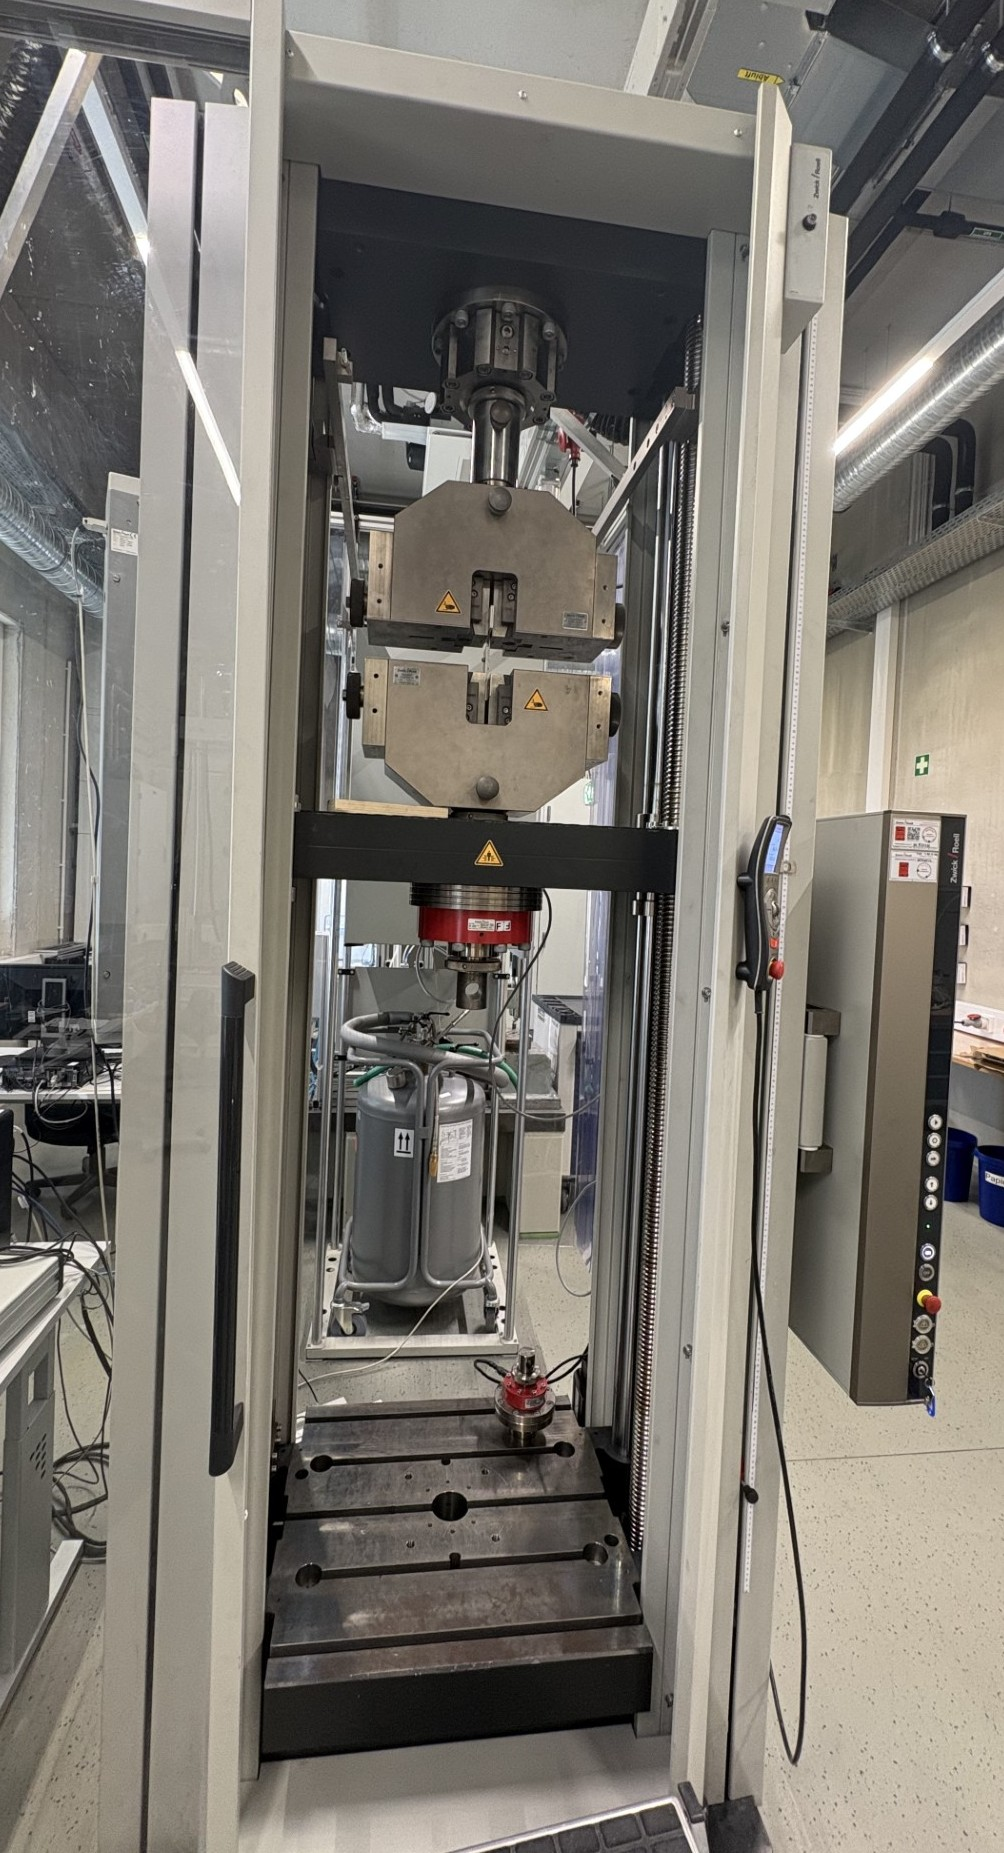
\includegraphics[width=0.27\textwidth]{Zugpruefmaschine_Zwick}
            \caption{Zugprüfmaschine Zwick/Roell Z250 (eigene Aufnahme).}
	  \label{fig:Zugpruefmaschine}
        \end{center}
    \end{figure}

Während des Versuchs wurden die aufgebrachte Kraft und der Traversenweg kontinuierlich aufgezeichnet.

	\section{Proben und Vorbereitung}
	Untersucht wurden drei Probenchargen mit jeweils fünf vernieteten Prüfkörpern. Alle
Proben bestanden aus zwei über eine Blindnietverbindung gefügten Blechen. Der
Bohrungsdurchmesser betrug bei sämtlichen Proben \SI{6.4}{\milli\metre}. Die Chargen
unterschieden sich hinsichtlich des Werkstoffs und der Blechdicken. Eine Übersicht ist
in \Tabref{tab:scherzug_probenchargen} angegeben.

\begin{table}[H]
    \centering
    \caption{Übersicht der im Scherzugversuch untersuchten Probenchargen.}
    \label{tab:scherzug_probenchargen}
    \resizebox{\textwidth}{!}{%
        \begin{tabular}{c c c c c}
            \hline
            Charge & Werkstoff & Blechdicke 1 & Blechdicke 2 & Probenanzahl \\
            \hline
            1 & AlMg3 & \SI{3}{\milli\metre} & \SI{3}{\milli\metre} & 5 \\
            2 & Chrom-Nickel-Stahl & \SI{2}{\milli\metre} & \SI{5}{\milli\metre} & 5 \\
            3 & Chrom-Nickel-Stahl & \SI{3}{\milli\metre} & \SI{3}{\milli\metre} & 5 \\
            \hline
        \end{tabular}%
    }
\end{table}

Die Aluminiumproben der ersten Charge sind exemplarisch in \Figref{fig:Zugproben Aluminium} dargestellt.

    \begin{figure}[H]
        \begin{center}
            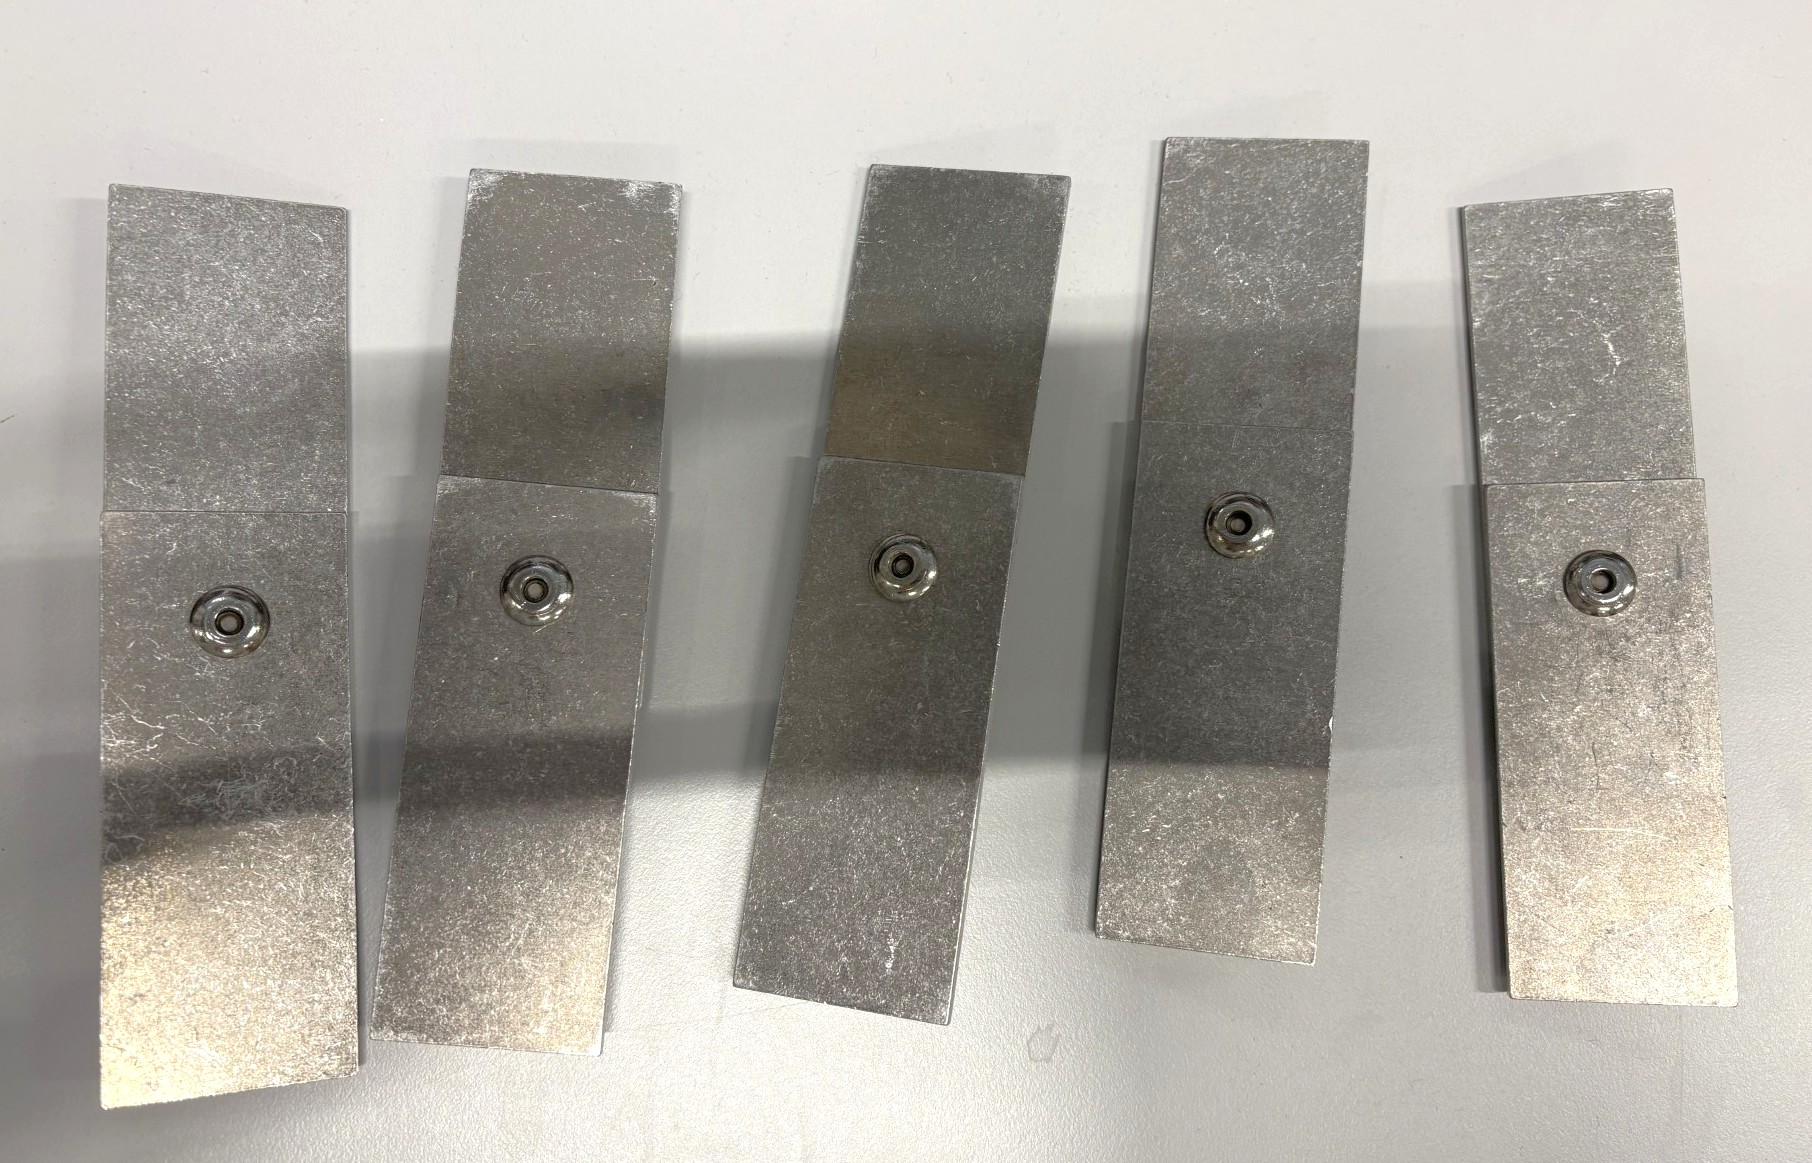
\includegraphics[width=0.75\textwidth]{Zugproben_Aluminium}
            \caption{Zugproben Aluminium.}
	  \label{fig:Zugproben Aluminium}
        \end{center}
    \end{figure}

Zur eindeutigen Zuordnung der Messdaten, Bruchbilder und Prüfprotokolle wurde für
sämtliche Proben eine einheitliche Probenbezeichnung verwendet. 
\clearpage
Die Bezeichnung \texttt{Z\_P05\_AlMg3\_3\_3mm\_D6.4\_kpl} enthält beispielsweise die Probenart, die Probennummer, den Werkstoff, die beiden Blechdicken, den Bohrungsdurchmesser und den
Bearbeitungsstatus. \\Diese eindeutige Benennung unterstützt die spätere standardisierte
Zuordnung und Weiterverarbeitung der Versuchsdaten.

	 \section{Durchführung}
	\subsection{Versuchsparameter}
	Damit die Nietverbindung möglichst ohne zusätzliche Biegebeanspruchung geprüft wird,
muss die Kraftlinie in der Ebene der Scherfuge liegen. Hierzu wurden Ausgleichsbleche
verwendet, deren Dicke an die jeweilige Probengeometrie angepasst war. Vor der
Versuchsdurchführung wurden die Kontaktflächen gereinigt und die Spannbacken parallel
sowie zentrisch ausgerichtet. Die zentrische und biegemomentarme Einspannung sowie die
gewählte Prüfgeschwindigkeit orientieren sich an den Vorgaben der DIN~EN~ISO~14589
für die mechanische Prüfung von Blindnieten~\cite[Seite~7]{Blindniete_Norm}.

Die wesentlichen Versuchsparameter sind in \Tabref{tab:scherzug_versuchsparameter} zusammengefasst.

\begin{table}[H]
    \centering
    \caption{Wesentliche Parameter der Scherzugversuche.}
    \label{tab:scherzug_versuchsparameter}
    \begin{tabular}{l l}
        \hline
        Prüfparameter & Eingestellter Wert \\
        \hline
        Prüfgeschwindigkeit & \SI{10}{\milli\metre\per\minute} \\
        Freie Prüflänge & \SI{80}{\milli\metre} \\
        Vorkraft & ca. \SI{120}{\newton} \\
        Abbruchkriterium & Versagen der Nietverbindung oder des Blechs \\
        \hline
    \end{tabular}
\end{table}

	\subsection{Versuchsablauf}
	
	Zu Beginn jedes Versuchs wurde die Probe zentrisch in die Spannbacken eingesetzt und
über die angepassten Ausgleichsbleche ausgerichtet. Für die erste Probencharge kamen
zunächst Spannbacken des Typs 8406 zum Einsatz. Da sich einzelne Proben beim Spannen
leicht verzogen, wurden für die beiden nachfolgenden Chargen größere Spannbacken des
Typs 8507 verwendet. Anschließend wurde die freie Prüflänge kontrolliert, die
Schutztür geschlossen und die Vorkraft von etwa \SI{120}{\newton} aufgebracht.

Nach dem Start der Messung wurde die Traverse mit konstanter Geschwindigkeit bewegt,
bis die Nietverbindung oder eines der Bleche versagte. Für jede Probe wurden der
Kraft-Weg-Verlauf, die Maximalkraft und die beobachtete Versagensart dokumentiert.
Diese Größen bilden die Grundlage der folgenden Auswertung.

	 \section{Auswertung}

Die Versuchsergebnisse werden mithilfe von Kraft-Weg-Diagrammen dargestellt. Für jede
Probe wird die Maximalkraft aus dem jeweiligen Kraftverlauf bestimmt. Zur Beschreibung
der Streuung innerhalb einer Charge werden der arithmetische Mittelwert, die
Standardabweichung und der Variationskoeffizient verwendet. Die zugehörigen
statistischen Grundlagen wurden in Kapitel~2 erläutert.

\subsection*{Charge 1: AlMg3, Blechdicken \SI{3}{\milli\metre}/\SI{3}{\milli\metre}}

Die Kraft-Weg-Verläufe der Aluminiumproben sind in
\Figref{fig:Diagramm_AlMg3_3} dargestellt. Für Probe~1 wurde kein verwertbarer
Messdatensatz gespeichert, weshalb die statistische Auswertung dieser Charge auf den
vier vollständig aufgezeichneten Versuchen basiert.
	  
    \begin{figure}[H]
        \begin{center}
            \includegraphics[width=0.8\textwidth]{Scherzugversuch_diagramm_AlMg3_3}
            \caption{Scherzugversuch - Proben 2-5 (AlMg3\_3\_3mm, D6.4).}
	  \label{fig:Diagramm_AlMg3_3}
        \end{center}
    \end{figure}
    
Die mittlere Maximalkraft beträgt 9770\,$N$. Mit einer
Standardabweichung von 40,8\,$N$ und einem Variationskoeffizienten von
0,42\,$\%$ weisen die aufgezeichneten Ergebnisse eine geringe Streuung auf.
Bei den geprüften Aluminiumproben trat das Versagen jeweils im Blech auf.

\subsection*{Charge 2: Chrom-Nickel-Stahl, Blechdicken
\SI{2}{\milli\metre}/\SI{5}{\milli\metre}}

Die Kraft-Weg-Verläufe der zweiten Charge sind in
\Figref{fig:Diagramm_CrNi2_5} abgebildet. Die Proben erreichten das Ausfallkriterium bei einem
geringeren Traversenweg als die Aluminiumproben. Bei allen fünf Proben trat ein
Nietbruch auf. Des Weiteren sind am Anfang der Kurven Zacken zu erkennen, die ihre Ursache vermutlich in einem leichten Verrutschen der Proben haben. 
    
Bei den Chrom-Nickel-Proben mit zwei und fünf Millimeter Blechstärke zeigt sich in \Figref{fig:Diagramm_CrNi2_5}, dass die Proben nach einem deutlich geringeren Weg bereits versagen. Des Weiteren sind am Anfang der Kurven Zacken zu erkennen, die ihre Ursache vermutlich darin haben, dass die Proben leicht verrutscht sind. 
        \begin{figure}[H]
        \begin{center}
            \includegraphics[width=0.8\textwidth]{Scherzugversuch_diagramm_CrNi2_5}
            \caption{Scherzugversuch - Proben 1-5 (CrNi\_2\_5mm, D6.4).}
	  \label{fig:Diagramm_CrNi2_5}
        \end{center}
    \end{figure}
Die mittlere Maximalkraft liegt bei 11000\,$N$, die Standardabweichung bei 328\,$N$ und der Variationskoeffizient bei 2,99\,$\%$. 

\subsection*{Charge 3: Chrom-Nickel-Stahl, Blechdicken
\SI{3}{\milli\metre}/\SI{3}{\milli\metre}}

Die dritte Charge weist die höchsten gemessenen Maximalkräfte auf. Die zugehörigen
Kraft-Weg-Verläufe sind in \Figref{fig:Diagramm_CrNi3_3} dargestellt. Auch bei
dieser Charge versagten sämtliche Proben durch einen Nietbruch.

            \begin{figure}[H]
        \begin{center}
            \includegraphics[width=0.8\textwidth]{Scherzugversuch_diagramm_CrNi3_3}
            \caption{Scherzugversuch - Proben 1-5 (CrNi\_3\_3mm, D6.4).}
	  \label{fig:Diagramm_CrNi3_3}
        \end{center}
    \end{figure}

Die mittlere Maximalkraft beträgt 14900\,$N$, die Standardabweichung 393\,$N$ und der Variationskoeffizient 2,63\,$\%$. 

\subsection*{Zusammenfassung und Einordnung}

\Tabref{tab:scherzug_ergebnisse} fasst die wesentlichen Ergebnisse der drei
Probenchargen zusammen.

\begin{table}[H]
    \centering
    \caption{Zusammenfassung der Ergebnisse der Scherzugversuche.}
    \label{tab:scherzug_ergebnisse}
    \resizebox{\textwidth}{!}{%
        \begin{tabular}{l c c c c}
            \hline
            Probencharge &
            mittlere Maximalkraft &
            Standardabweichung &
            Variationskoeffizient &
            Versagensart \\
            \hline
            AlMg3, 3/3 mm &
            \SI{9770}{\newton} &
            \SI{40.8}{\newton} &
            \SI{0.42}{\percent} &
            Blechversagen \\
            CrNi, 2/5 mm &
            \SI{11000}{\newton} &
            \SI{328}{\newton} &
            \SI{2.99}{\percent} &
            Nietbruch \\
            CrNi, 3/3 mm &
            \SI{14900}{\newton} &
            \SI{393}{\newton} &
            \SI{2.63}{\percent} &
            Nietbruch \\
            \hline
        \end{tabular}%
    }
\end{table}

 Die Ergebnisse zeigen, dass sich sowohl die maximal übertragbare Kraft als auch die
Versagensart in Abhängigkeit von Werkstoff und Blechdicken unterscheiden. Ein
unmittelbarer werkstofflicher Vergleich allein anhand des Traversenwegs ist jedoch nur
eingeschränkt möglich, da sich neben dem Werkstoff auch die Geometrie und die
Versagensart der Chargen unterscheiden.

Für die nachfolgenden Wöhlerversuche ist insbesondere die statische Tragfähigkeit der
jeweils untersuchten Nietverbindung relevant. Die im Scherzugversuch ermittelten
Maximalkräfte dienen daher als obere Orientierungsgröße für die Festlegung der
dynamischen Lastniveaus. Die Lasten des Wöhlerversuchs werden unterhalb dieser
statischen Versagenslasten gewählt, sodass nicht ein unmittelbares statisches Versagen,
sondern das Ermüdungsverhalten der Verbindung untersucht wird. Die vollständigen
Prüfprotokolle der Scherzugversuche sind in \Anhref{anhang:pruefprotokoll} enthalten.



    %-----------------------------------------------------------------------
\chapter{Layout und Aufbau der Ausarbeitung}%\label{chap:kap1}
%-----------------------------------------------------------------------




    %% Kapitel
    %
% Ostbayerische Technische Hochschule Regensburg (OTH)
% Fakultät Maschinenbau
% Prof. Dr.-Ing. Marcus Wagner
%
% Vorlage und Hinweise für die Erstellung von Abschlussarbeiten
% Inhaltliche Angaben basieren zum Teil auf Vorlagen von Prof. Ehrlich LFT
%
% v1 August 2017
%-----------------------------------------------------------------------
\chapter{Abbildungen, Tabellen, Gleichungen}%\label{chap:kap1}
%-----------------------------------------------------------------------


    %% Kapitel
    %s %
% Ostbayerische Technische Hochschule Regensburg (OTH)
% Fakultät Maschinenbau
% Prof. Dr.-Ing. Marcus Wagner
%
% Vorlage und Hinweise für die Erstellung von Abschlussarbeiten
% Inhaltliche Angaben basieren zum Teil auf Vorlagen von Prof. Ehrlich LFT
%
% v1 August 2017
%-----------------------------------------------------------------------
\chapter{Literatur}%\label{chap:kap1}
%-----------------------------------------------------------------------

@online{webseite,
 	author = {{Technology Arts Sciences TH Kölln}},
	date = {2018, April}
 	title = {{Prüfmaschine zur Messung des Ermüdungsverhaltens von Bauteilen}},
	url = {https://www.th-koeln.de/hochschule/pruefmaschine-zur-messung-des-ermuedungsverhaltens-von-bauteilen_54301.php},
	urldate  = {2026-04-01}
}





    %\nocite{bibid}
    %% Literaturverzeichnis ausgeben
    \printbibliography[heading=bibnumbered] %Diese Option nummeriert das Litvezeichnsi

    %% Abkürzungsverzeichnisse, wenn gewünscht, ansonsten die folgende Zeile auskommentieren. 
    \chapter{Glossar} \printglossaries % Entries in file chapters/gloassar are printed at this position. Used für abbreviations and explanations of symbols
    % Einzeln 
    %\printglossary[type=\acronymtype, title={Abkürzungsverzeichnis}] %Abkürzungen
    %\printglossary[type=symbolslist, title={Formelzeichen}]
    %\printglossary[type=indexlist, title={Indizes}]
    %\printglossary[type=operatorlist,style=super]


    %% Wenn notwendig Anhangkapitel hier einfügen
    \appendix
    %-----------------------------------------------------------------------
\chapter{Anhangkapitel}\label{chap:anhang}
%-----------------------------------------------------------------------
\section{Prüfprotokolle} \label{anhang:pruefprotokoll}

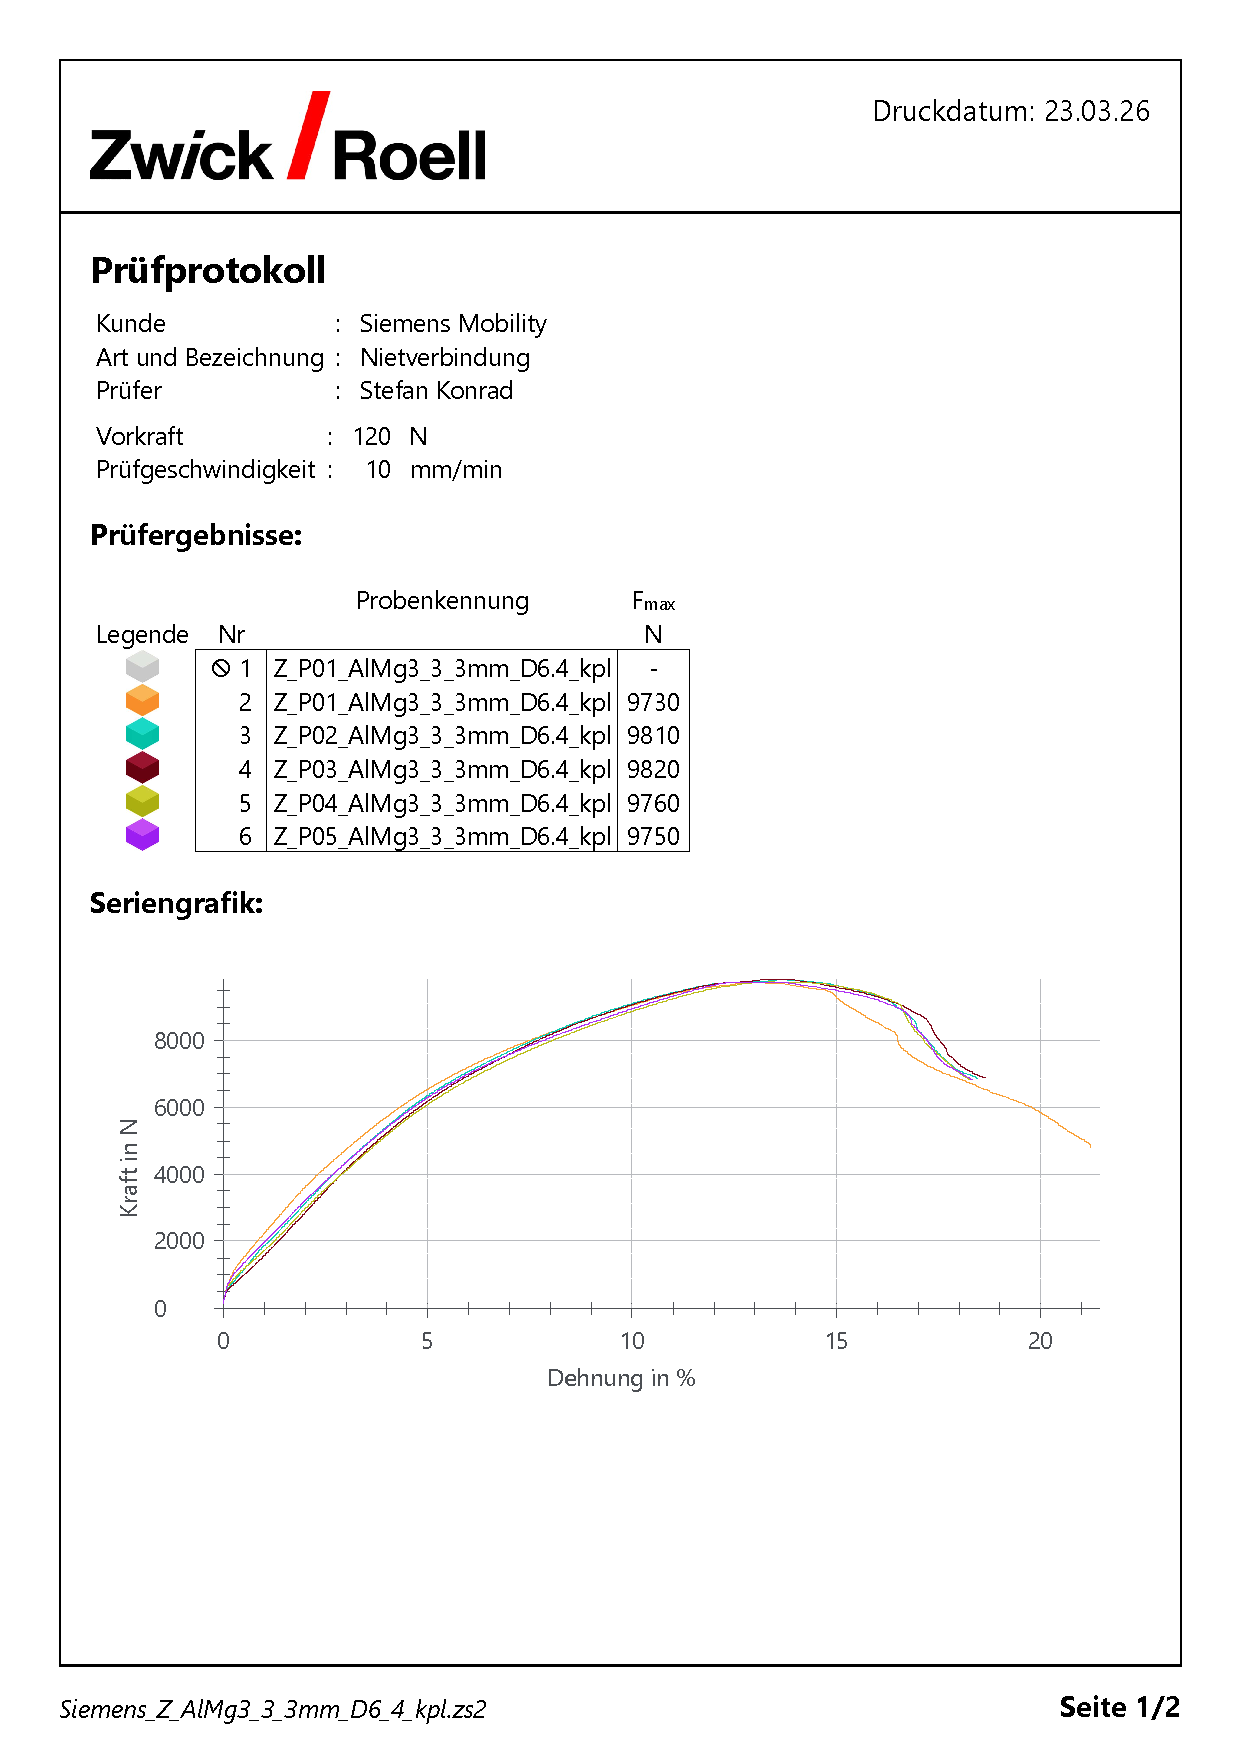
\includepdf[pages=-, scale=0.8, pagecommand={\thispagestyle{headings}}]{Siemens_Z_AlMg3_3_3mm.pdf}

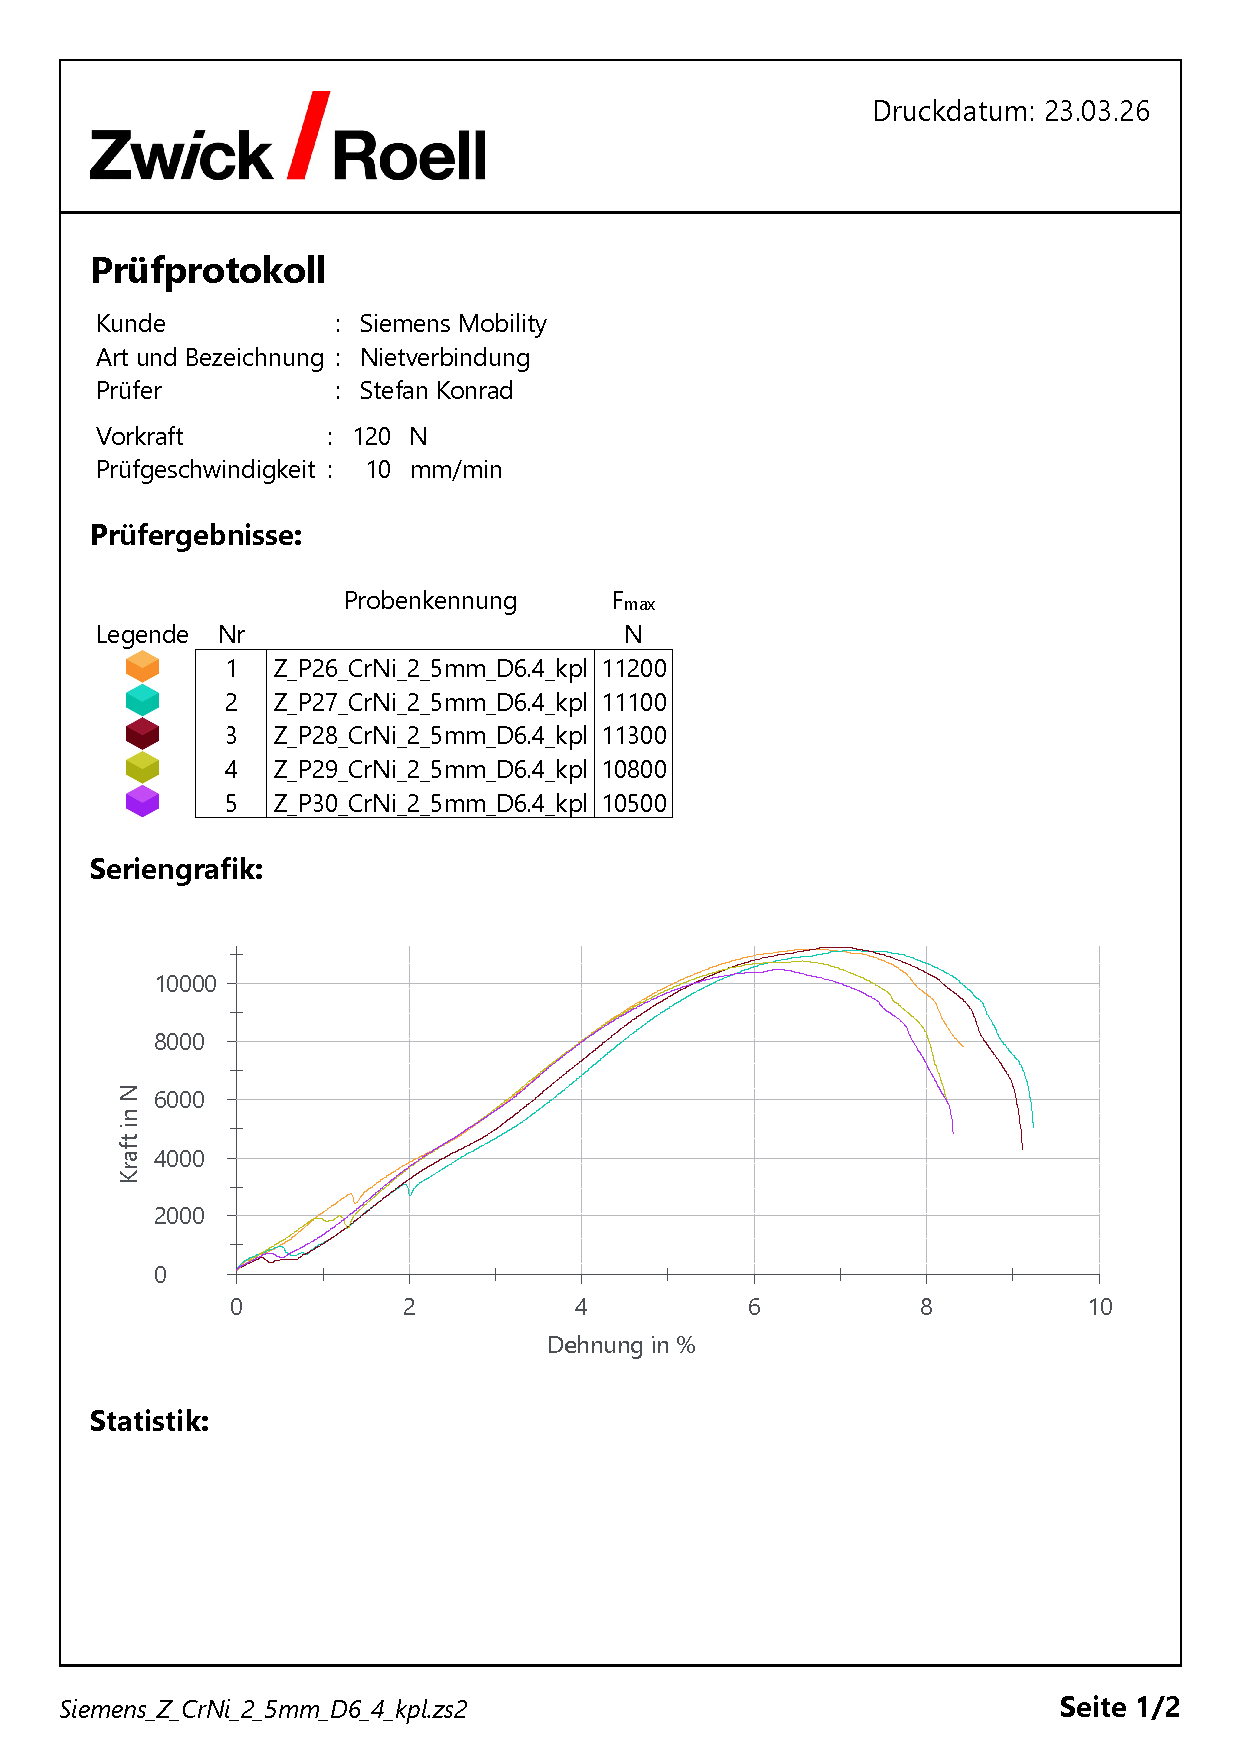
\includepdf[pages=-, scale=0.8, pagecommand={\thispagestyle{headings}}]{Siemens_Z_CrNi_2_5mm.pdf}

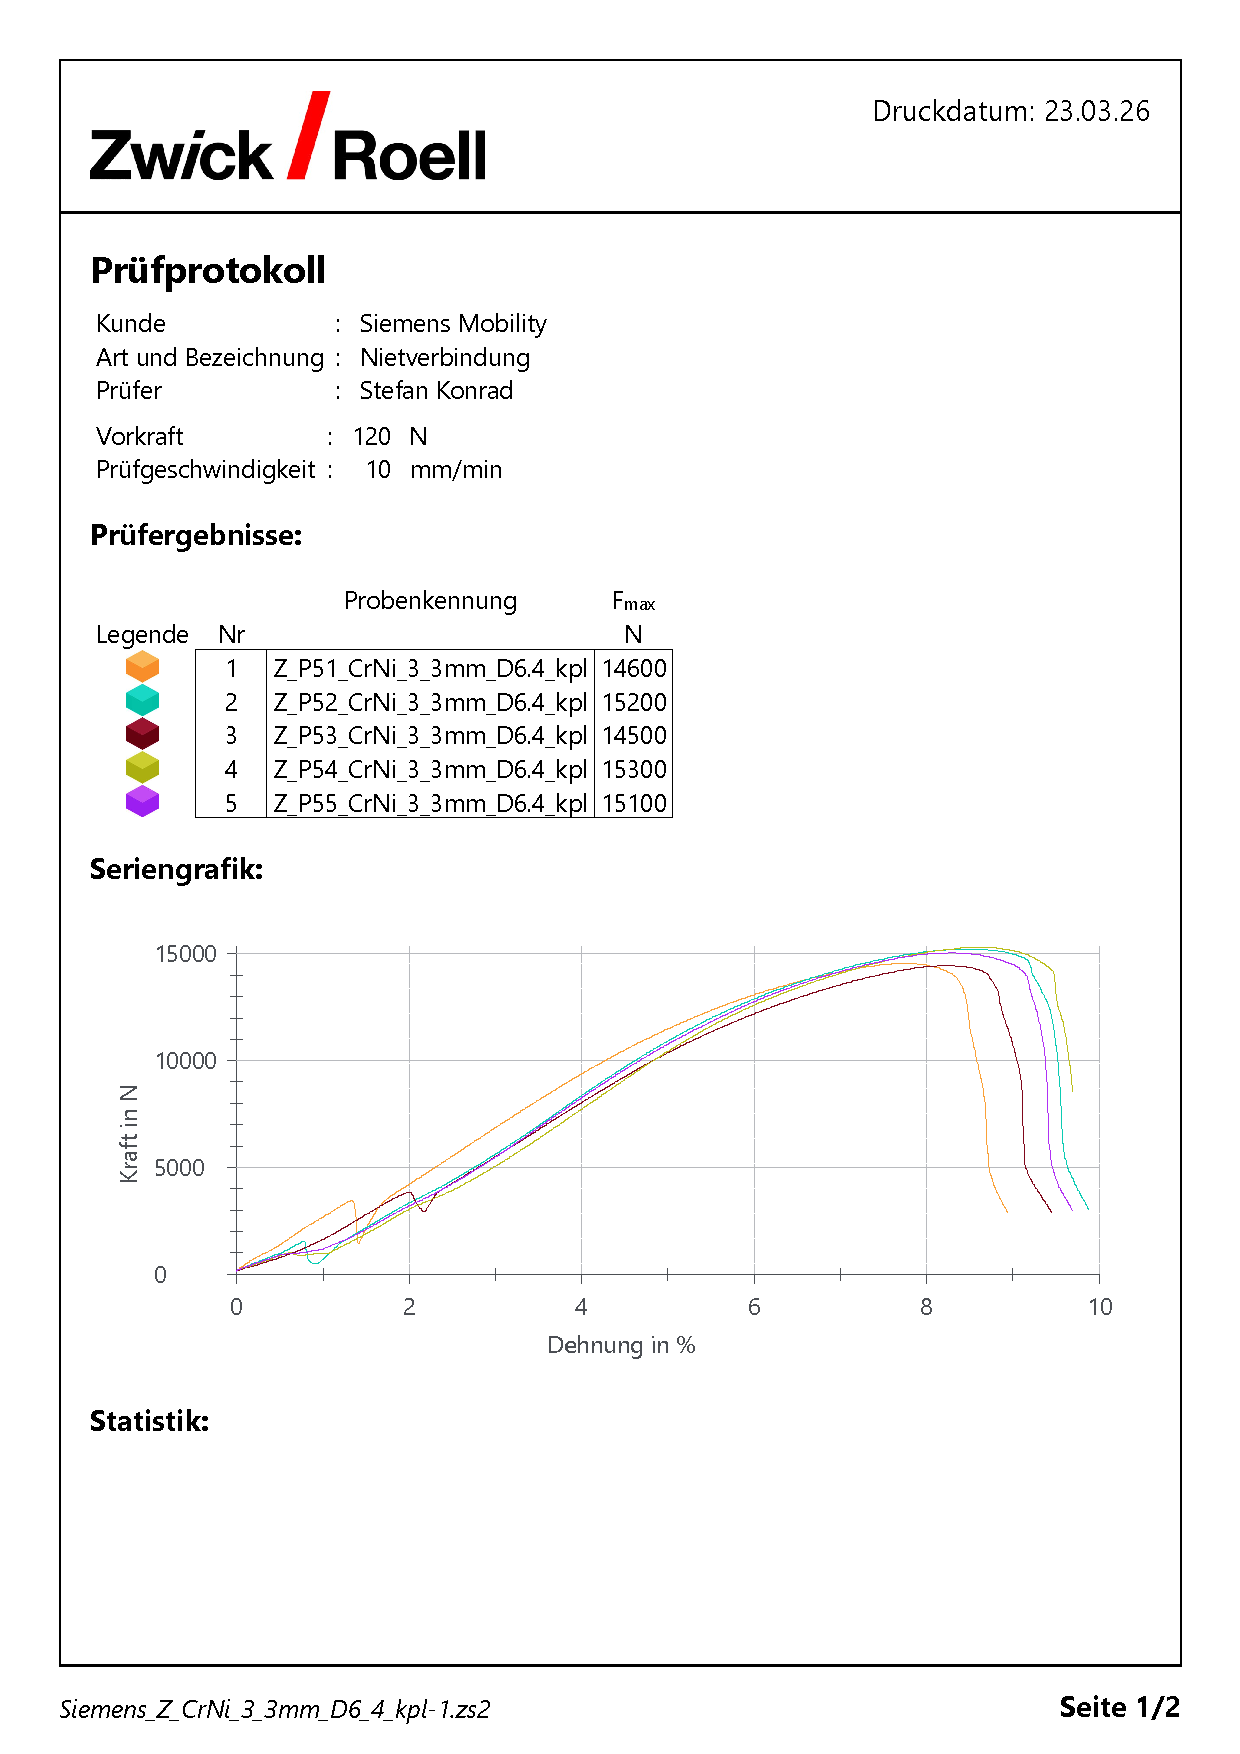
\includepdf[pages=-, scale=0.8, pagecommand={\thispagestyle{headings}}]{Siemens_Z_CrNi_3_3mm.pdf}










\end{document} 